\documentclass[aspectratio=169]{beamer}
%\usetheme{CambridgeUS}
%\usecolortheme{beaver}

%\usefonttheme{serif}
%\usepackage{helvet}

\usefonttheme{serif}     % Font theme: serif
%\usepackage{ccfonts}     % Font family: Concrete Math
\usepackage[T1]{fontenc} % Font encoding: T1

\setbeamersize{text margin left=42pt,text margin right=42pt} 
\setbeamertemplate{navigation symbols}{}
\setbeamertemplate{itemize items}[default]

\beamertemplatenavigationsymbolsempty

\definecolor{fore}{RGB}{51,51,51}
\definecolor{back}{RGB}{255, 254, 250}
\definecolor{title}{RGB}{ 255, 15, 0}
\definecolor{links}{RGB}{18, 168, 255}

\setbeamercolor{titlelike}{fg=title}
\setbeamercolor{normal text}{fg=fore,bg=back}
\setbeamercolor{alerted text}{fg=title}
\setbeamercolor{itemize item}{fg=title}
\setbeamercolor{enumerate item}{fg=title}
\hypersetup{colorlinks,urlcolor=links}

% for code https://kbroman.org/blog/2013/10/07/better-looking-latexbeamer-slides/
\usepackage{listings}
\definecolor{keywords}{RGB}{255,0,90}
\definecolor{comments}{RGB}{60,179,113}
\lstset{language=Python,
keywordstyle=color{keywords},
commentstyle=color{comments}emph}

% fonts
\usepackage[sc]{mathpazo}


% title info
\title{\textbf{Cars, Roads, \& Highways}}
\subtitle{\textbf{GGR424 - Transportation Geography \& Planning}}
\author{Jeff Allen}
\institute{University of Toronto}
\date{January 17, 2022}


\begin{document}
	
\begin{frame}
	\titlepage	
\end{frame}



\begin{frame}
\textbf{Today:}
\begin{itemize}
	\item Cars \& Highways - A Brief History
	\item Accessibility \& Mobility
	\item Road Networks \& Hierarchy
	\item Costs \& Benefits of Auto-mobility
	\item Transportation planning/services in Ontario
\end{itemize}
\end{frame}






\begin{frame}
	
	Toronto, before the car (1890s)
	
	\begin{figure}
		\centering
		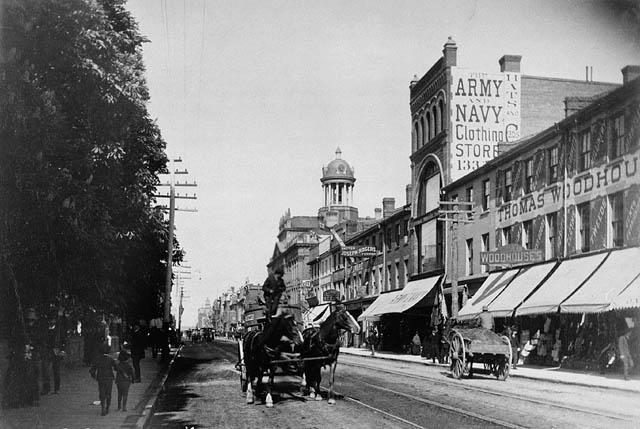
\includegraphics[width=0.8\linewidth]{images/king_east_1890s.jpg}
		
	\end{figure}
	
	\tiny{\url{https://upload.wikimedia.org/wikipedia/commons/d/dc/King_Street_East_1890s.jpg}}
\end{frame}




\begin{frame}
	
	\begin{figure}
		\centering
		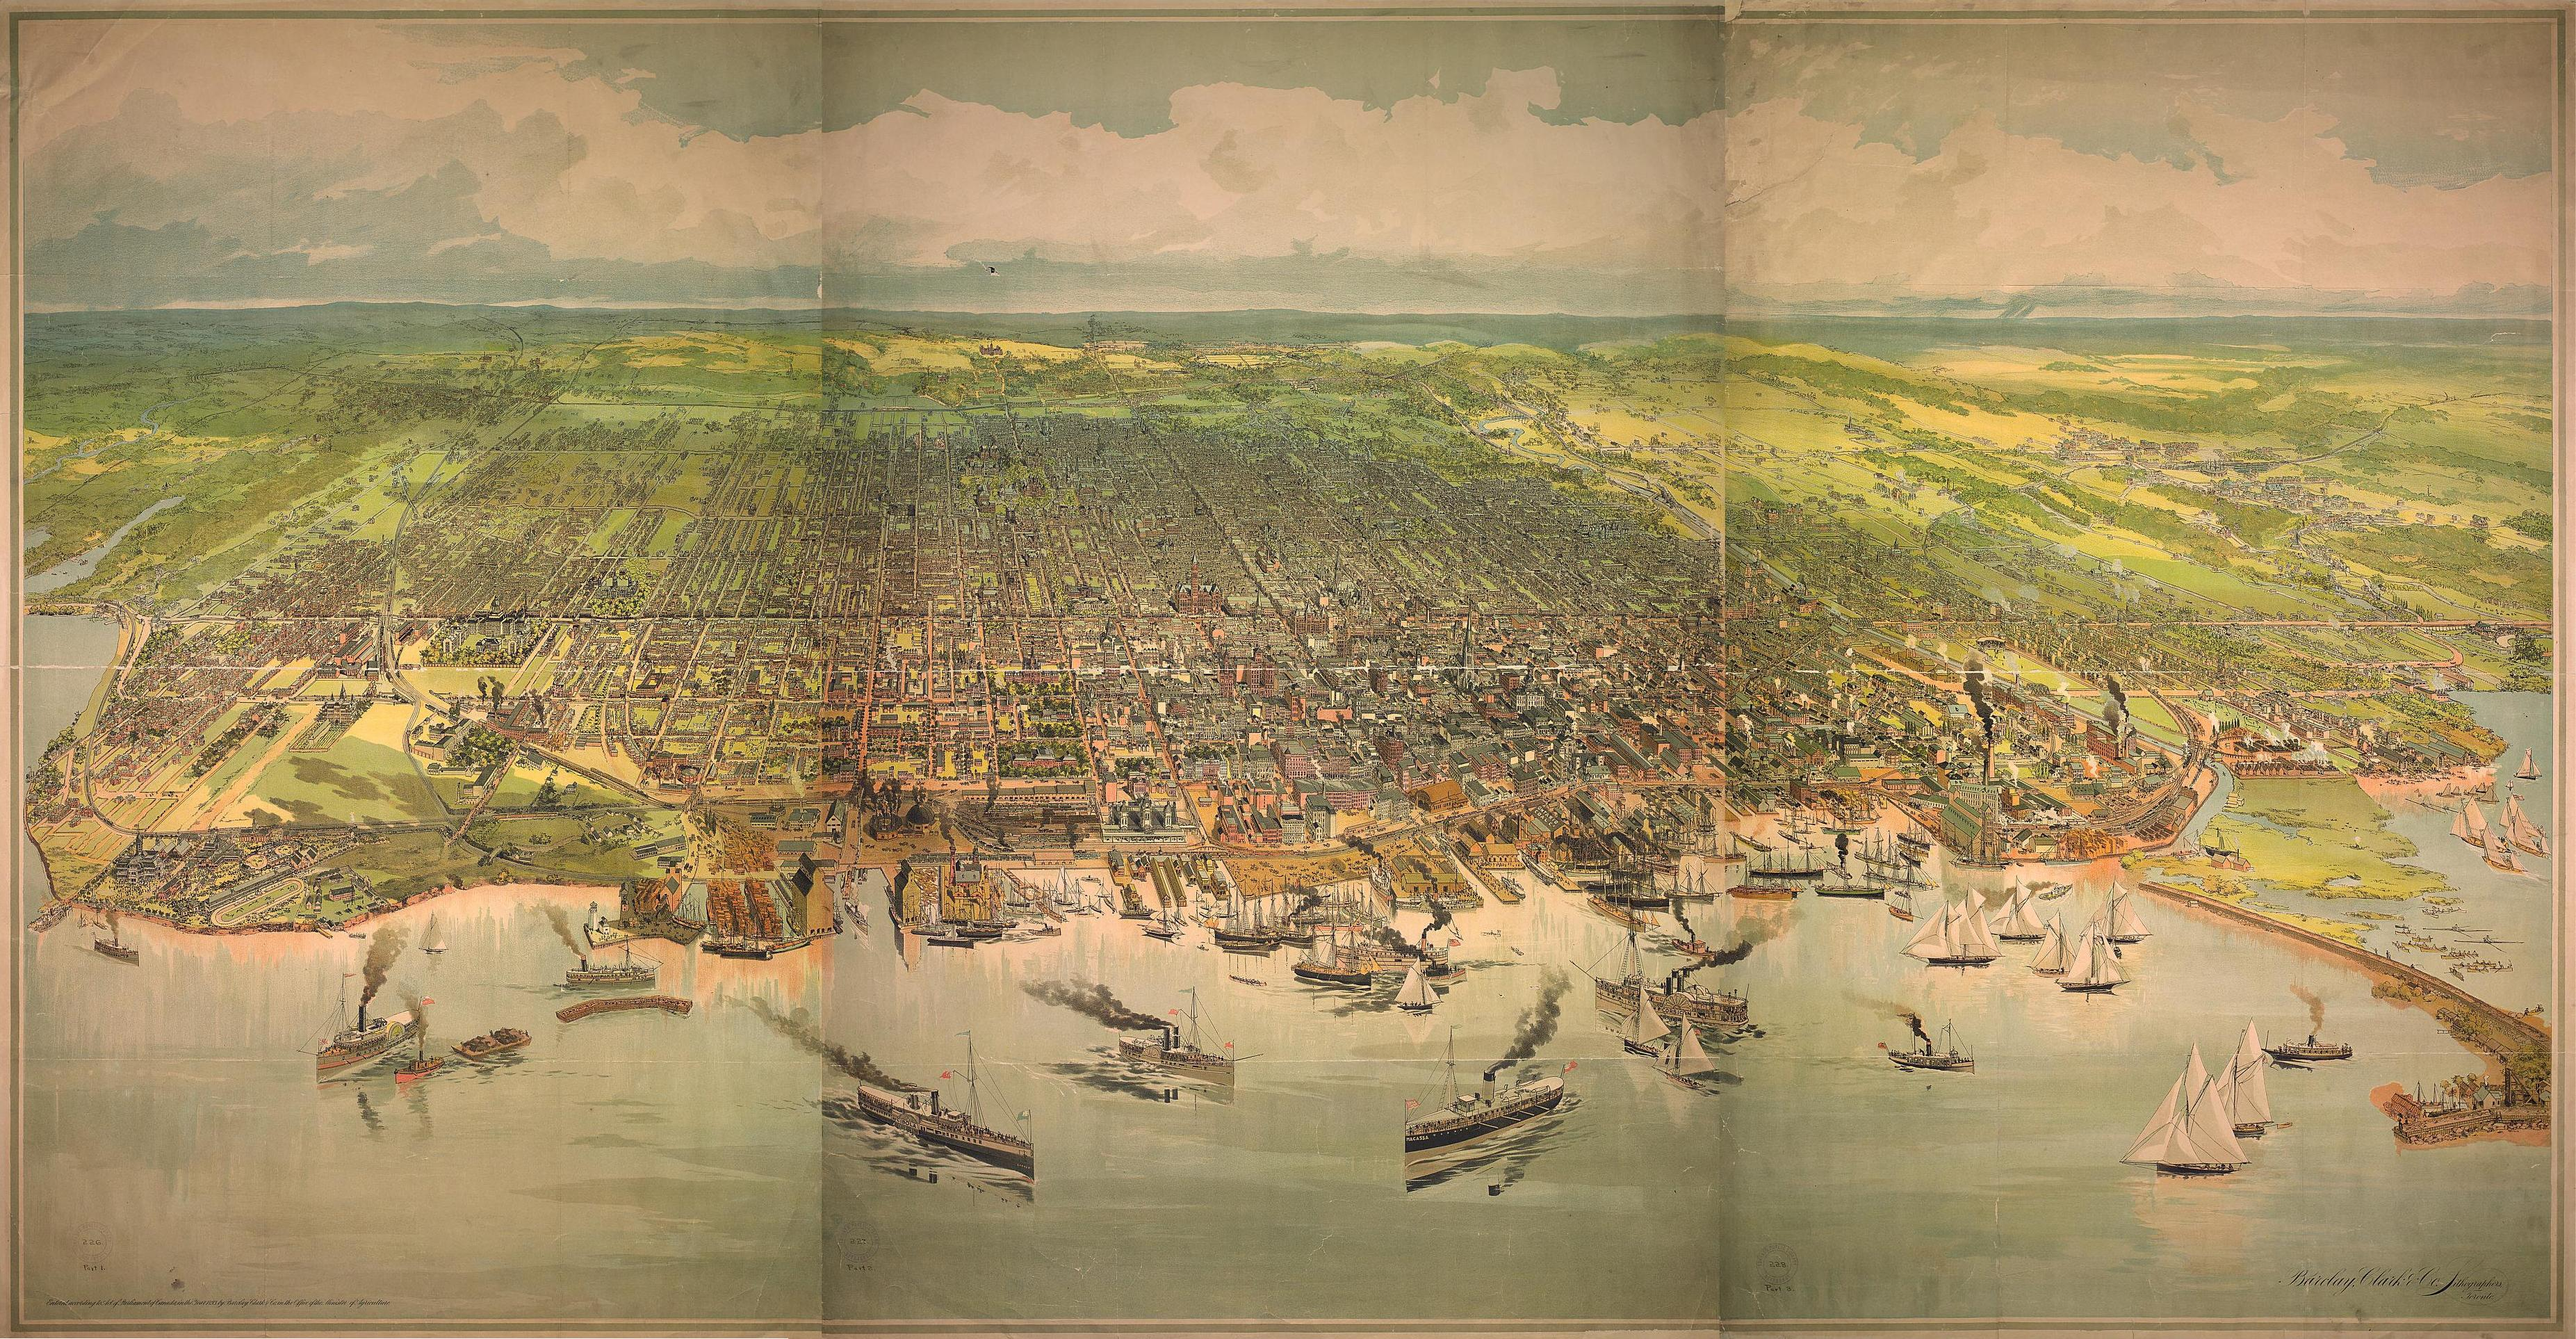
\includegraphics[width=1.1\linewidth]{images/toronto_1893.jpg}
		
	\end{figure}
	\tiny{Via UofT Map \& Data Library \url{https://maps.library.utoronto.ca/datapub/digital/NG/historicTOmaps/1893BarclayClark.Chromolithograph_of_City_of_Toronto.JPG}}
	
\end{frame}










\begin{frame}
	
	In 1911...
	
	\begin{figure}
		\centering
		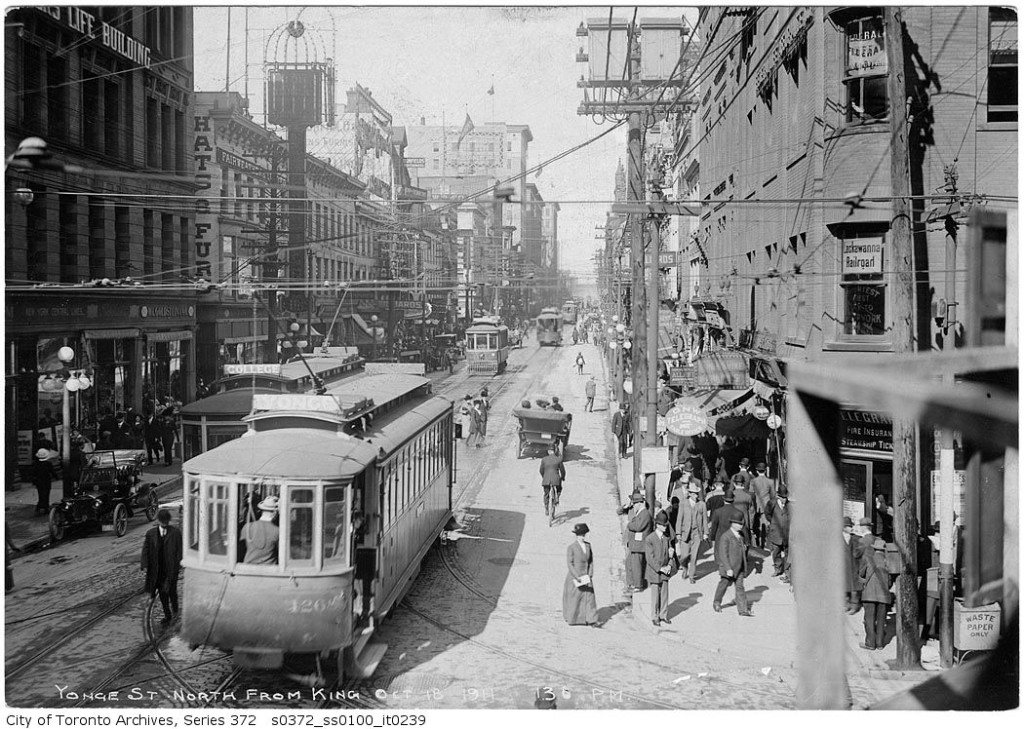
\includegraphics[width=0.8\linewidth]{images/yonge-north-from-king-1911.jpg}
		
	\end{figure}

	% what see?
	
\end{frame}



\begin{frame}
	
	
	Increase in car ownership and auto-mobility in Canada
	
	- \textit{What's driving these trends?}
	
	\begin{figure}
		\centering
		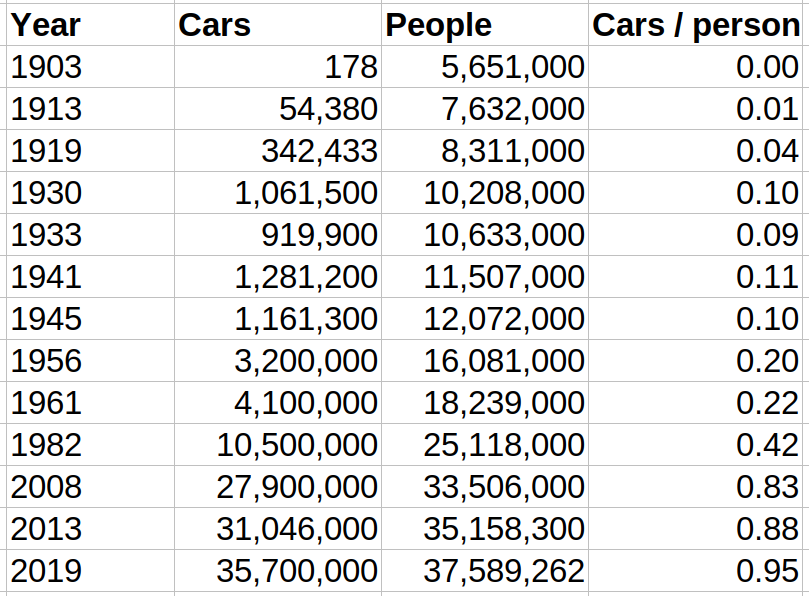
\includegraphics[width=0.6\linewidth]{images/cars_ppl_canada.png}
		
	\end{figure}
	
	\tiny{
		Sources:
		
		- McNally, Larry. “Roads, Streets, and Highways,” in Building Canada: a history of public	works
		
		- \url{https://www.statcan.gc.ca/en/topics-start/automotive}	
}
	
\end{frame}




\begin{frame}
	
	\textbf{Personal Benefits of Cars:}
	
	\vspace{3mm}
	
	\begin{itemize}
		\item Improved \textit{\textbf{Mobility}} and \textit{\textbf{Accessibility}}
		\item Increased Capacity for \textit{\textbf{Activity Participation}}
		\item Convenience, Freedom, etc.
		\item i.e. can decrease the negative \textbf{\textit{Utility}} of travel
	\end{itemize}
	
	Overall, trends show increasing \textbf{\textit{Demand}} for car-based travel over the past 120 years
	
\end{frame}




\begin{frame}
	
	e.g. having a car is associated with employment, job retention, and earning more money:
	
	\begin{figure}
		\centering
		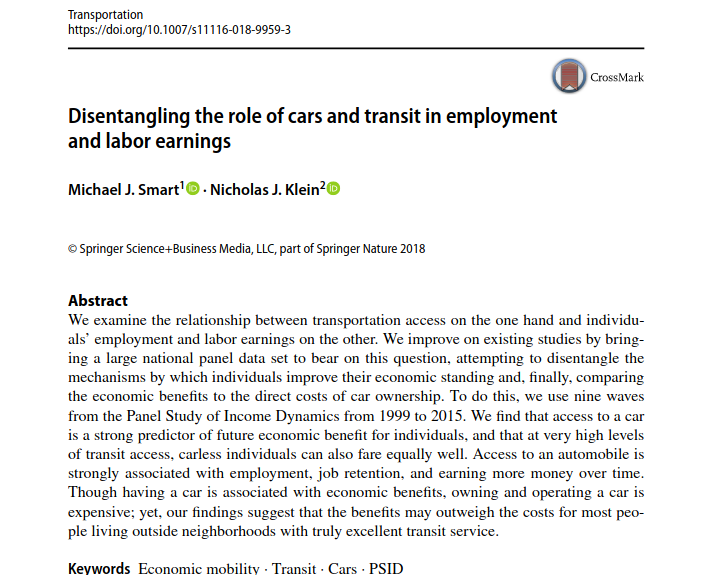
\includegraphics[width=0.6\linewidth]{images/klein_smart_cars.png}
		
	\end{figure}
	
	\tiny{\url{https://link.springer.com/article/10.1007/s11116-018-9959-3}}
	
	
\end{frame}	




\begin{frame}
	\textbf{Key Concepts in Urban Transportation}
	\normalsize
	\vspace{4mm}
	\begin{itemize}
		\item Travel Demand
		\item Activity Participation
		\item Utility
		\item Travel Behaviour
		\item \textbf{\underline{Mobility}}
		\item \textbf{\underline{Accessibility}}
		% \item Transport \& Land Use
		% \item Mobility VS Accessibility
	\end{itemize}
\end{frame}



\begin{frame}
	
	\textbf{Mobility}
	\begin{itemize}
		\item \textit{The ease of travelling}
		\item Measured via speeds and throughput
	\end{itemize}
	
	\textbf{Accessibility}
	\begin{itemize}
		\item \textit{The ease of reaching destinations}
		\item Depends on mobility, but also land-use (i.e. the proximity of destinations)
		\item Measurements: 
		\begin{itemize}
			\item minimum travel time to reach X
			\item how many Y can you reach in Z minutes
			\item combined indices (e.g. walkscore)
			\item more on this in Week 5
		\end{itemize}
	\end{itemize}
	
\end{frame}





\begin{frame}
	
	\textbf{Mobility}
	
	\vspace{4mm}
	
	Good Mobility \hspace{38mm} Bad Mobility
	
	
	\begin{figure}
		\centering
		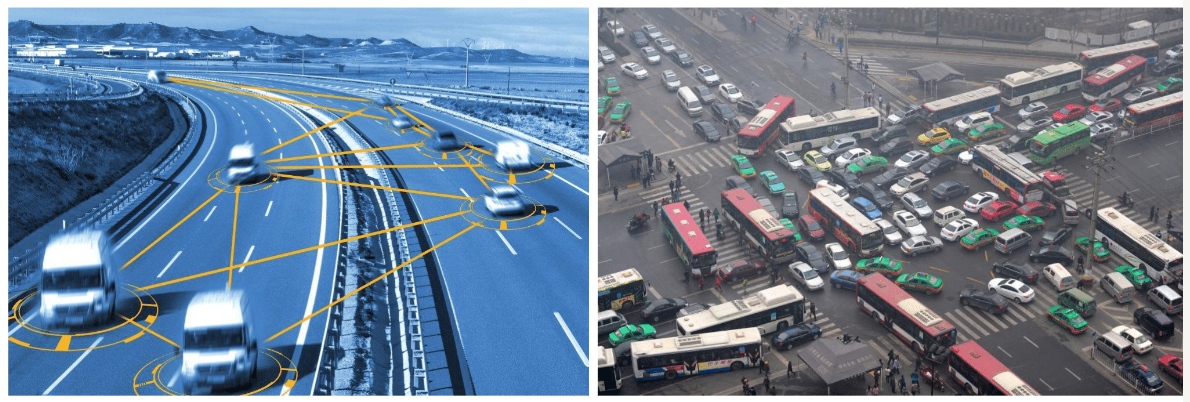
\includegraphics[width=1\linewidth]{images/mobility-good-bad.png}
		
	\end{figure}
	
	Transportation planning has historically focused on improving (auto)mobility
	
	
\end{frame}


\begin{frame}
	
	
	\vspace{4mm}
	
	\textbf{Planning \& Design Strategies for Improving (Auto)Mobility:}
	
	\vspace{2mm}
	
	\begin{itemize}
		\item Older strategies, e.g.
		\begin{itemize}
			\item Building new roads/highways
			\item Increase speeds/capacity of existing roads/highways
			\item Cheaper gas
			\item Lots of parking
		\end{itemize}
		
		\item Newer strategies, e.g.
		\begin{itemize}
			\item Real-time data (e.g. Google Maps, Waze, etc.)
			\item ITS (Intelligent Transportation Systems)
			\item Autonomous/Connected vehicles
		\end{itemize}
	\end{itemize}
	
\end{frame}








	
	


\begin{frame}
	
	Improving (auto)mobility - Public Infrastructure
	
	\begin{figure}
		\centering
		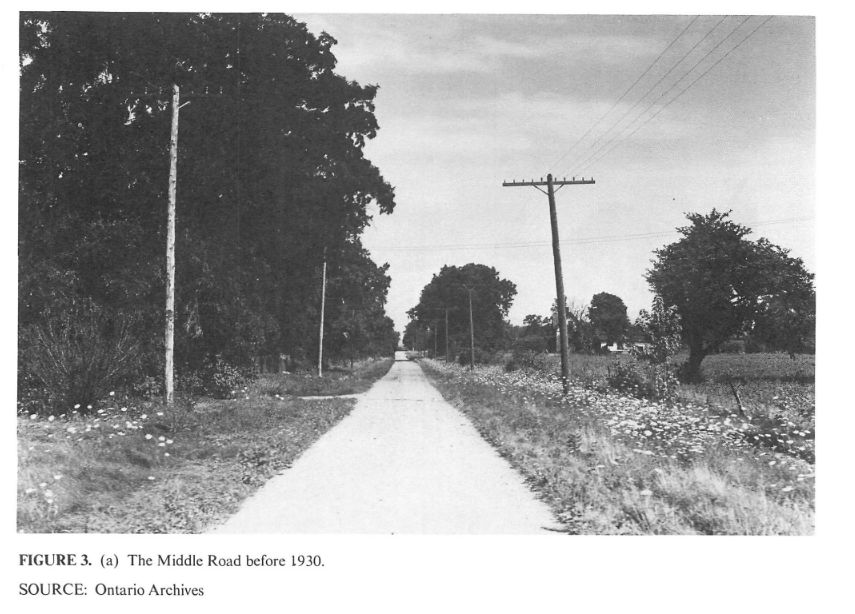
\includegraphics[width=0.8\linewidth]{images/qew_1930.png}
		
	\end{figure}
	\tiny{The Queen Elizabeth Way: Public Utility Versus Public Space = \url{https://www.erudit.org/en/journals/uhr/1900-v1-n1-uhr0860/1018953ar.pdf}}
	
\end{frame}




\begin{frame}
	
	\begin{figure}
		\centering
		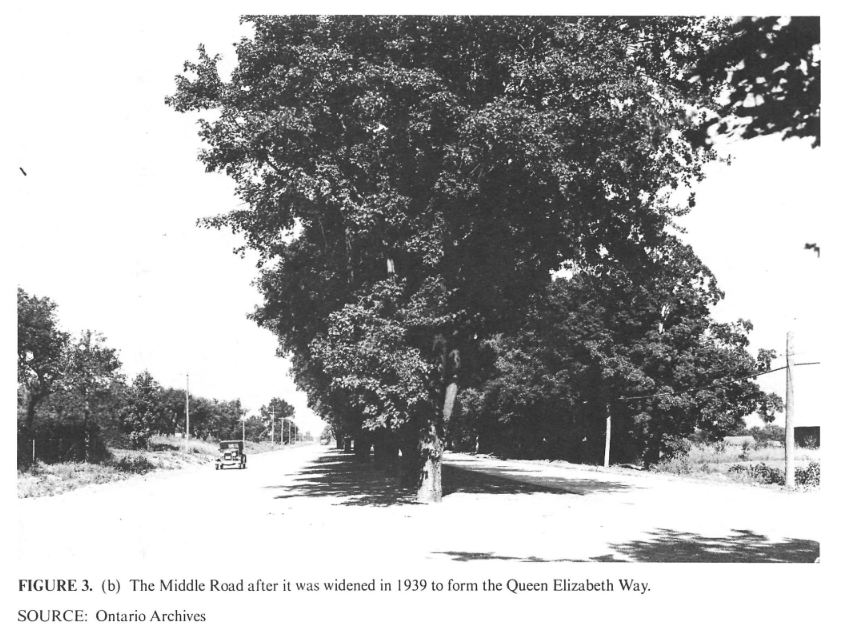
\includegraphics[width=0.8\linewidth]{images/qew_1939.png}
		
	\end{figure}
	\tiny{The Queen Elizabeth Way: Public Utility Versus Public Space = \url{https://www.erudit.org/en/journals/uhr/1900-v1-n1-uhr0860/1018953ar.pdf}}
	
\end{frame}


\begin{frame}
	
	\begin{figure}
		\centering
		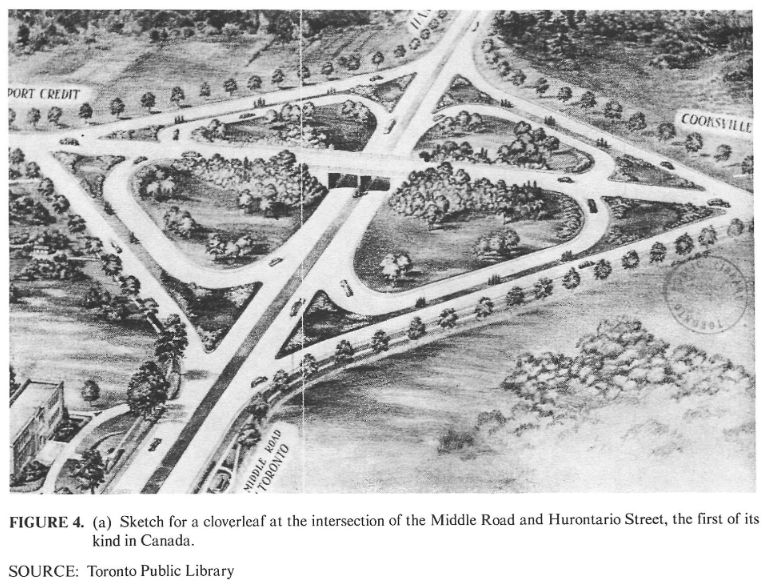
\includegraphics[width=0.8\linewidth]{images/qew_highway10.png}
		
	\end{figure}
	\tiny{The Queen Elizabeth Way: Public Utility Versus Public Space = \url{https://www.erudit.org/en/journals/uhr/1900-v1-n1-uhr0860/1018953ar.pdf}}
	
\end{frame}



\begin{frame}
	
	\begin{figure}
		\centering
		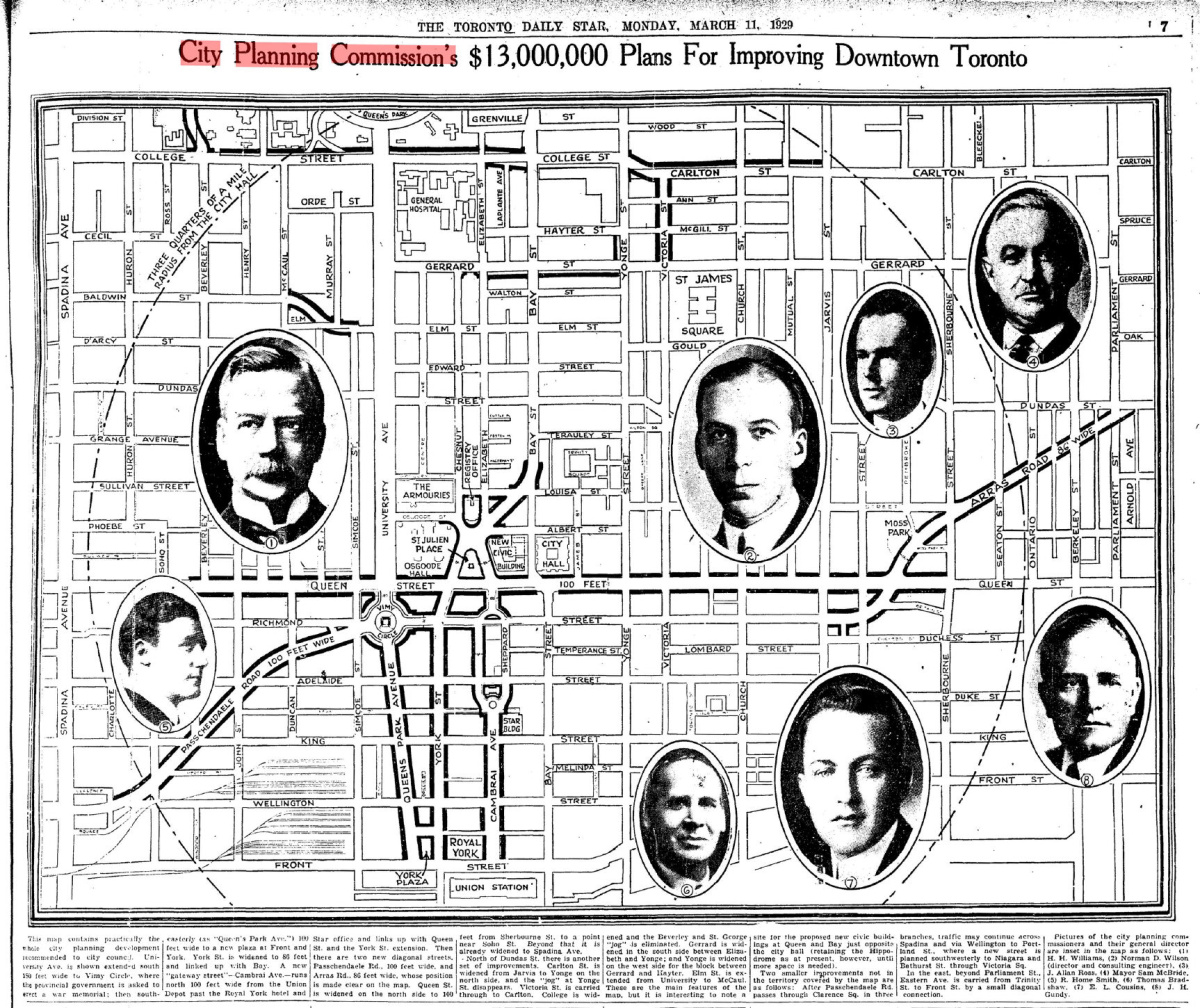
\includegraphics[width=0.7\linewidth]{images/toronto_road_plans_1929.jpg}
		
	\end{figure}
	
	
\end{frame}



\begin{frame}
	
	\begin{figure}
		\centering
		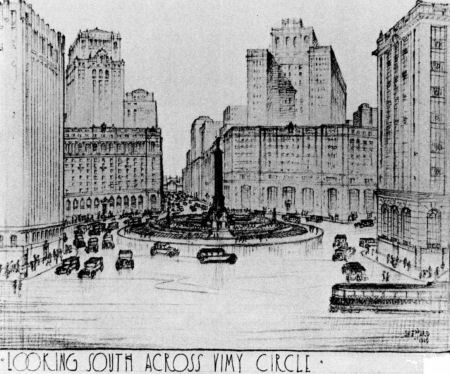
\includegraphics[width=0.7\linewidth]{images/vimy_circle.jpg}
		
		
		
	\end{figure}

\tiny{Source: Hayes (2008) Historical Atlas of Toronto}
	
	
\end{frame}


\begin{frame}
	
	\begin{figure}
		\centering
		\includegraphics[width=1\linewidth]{images/toronto_plan_1959.jpg}
		
	\end{figure}
	
	
	\tiny{1959 - Source: U of T Map and Data Library}
	
\end{frame}






\begin{frame}
	
	\begin{figure}
		\centering
		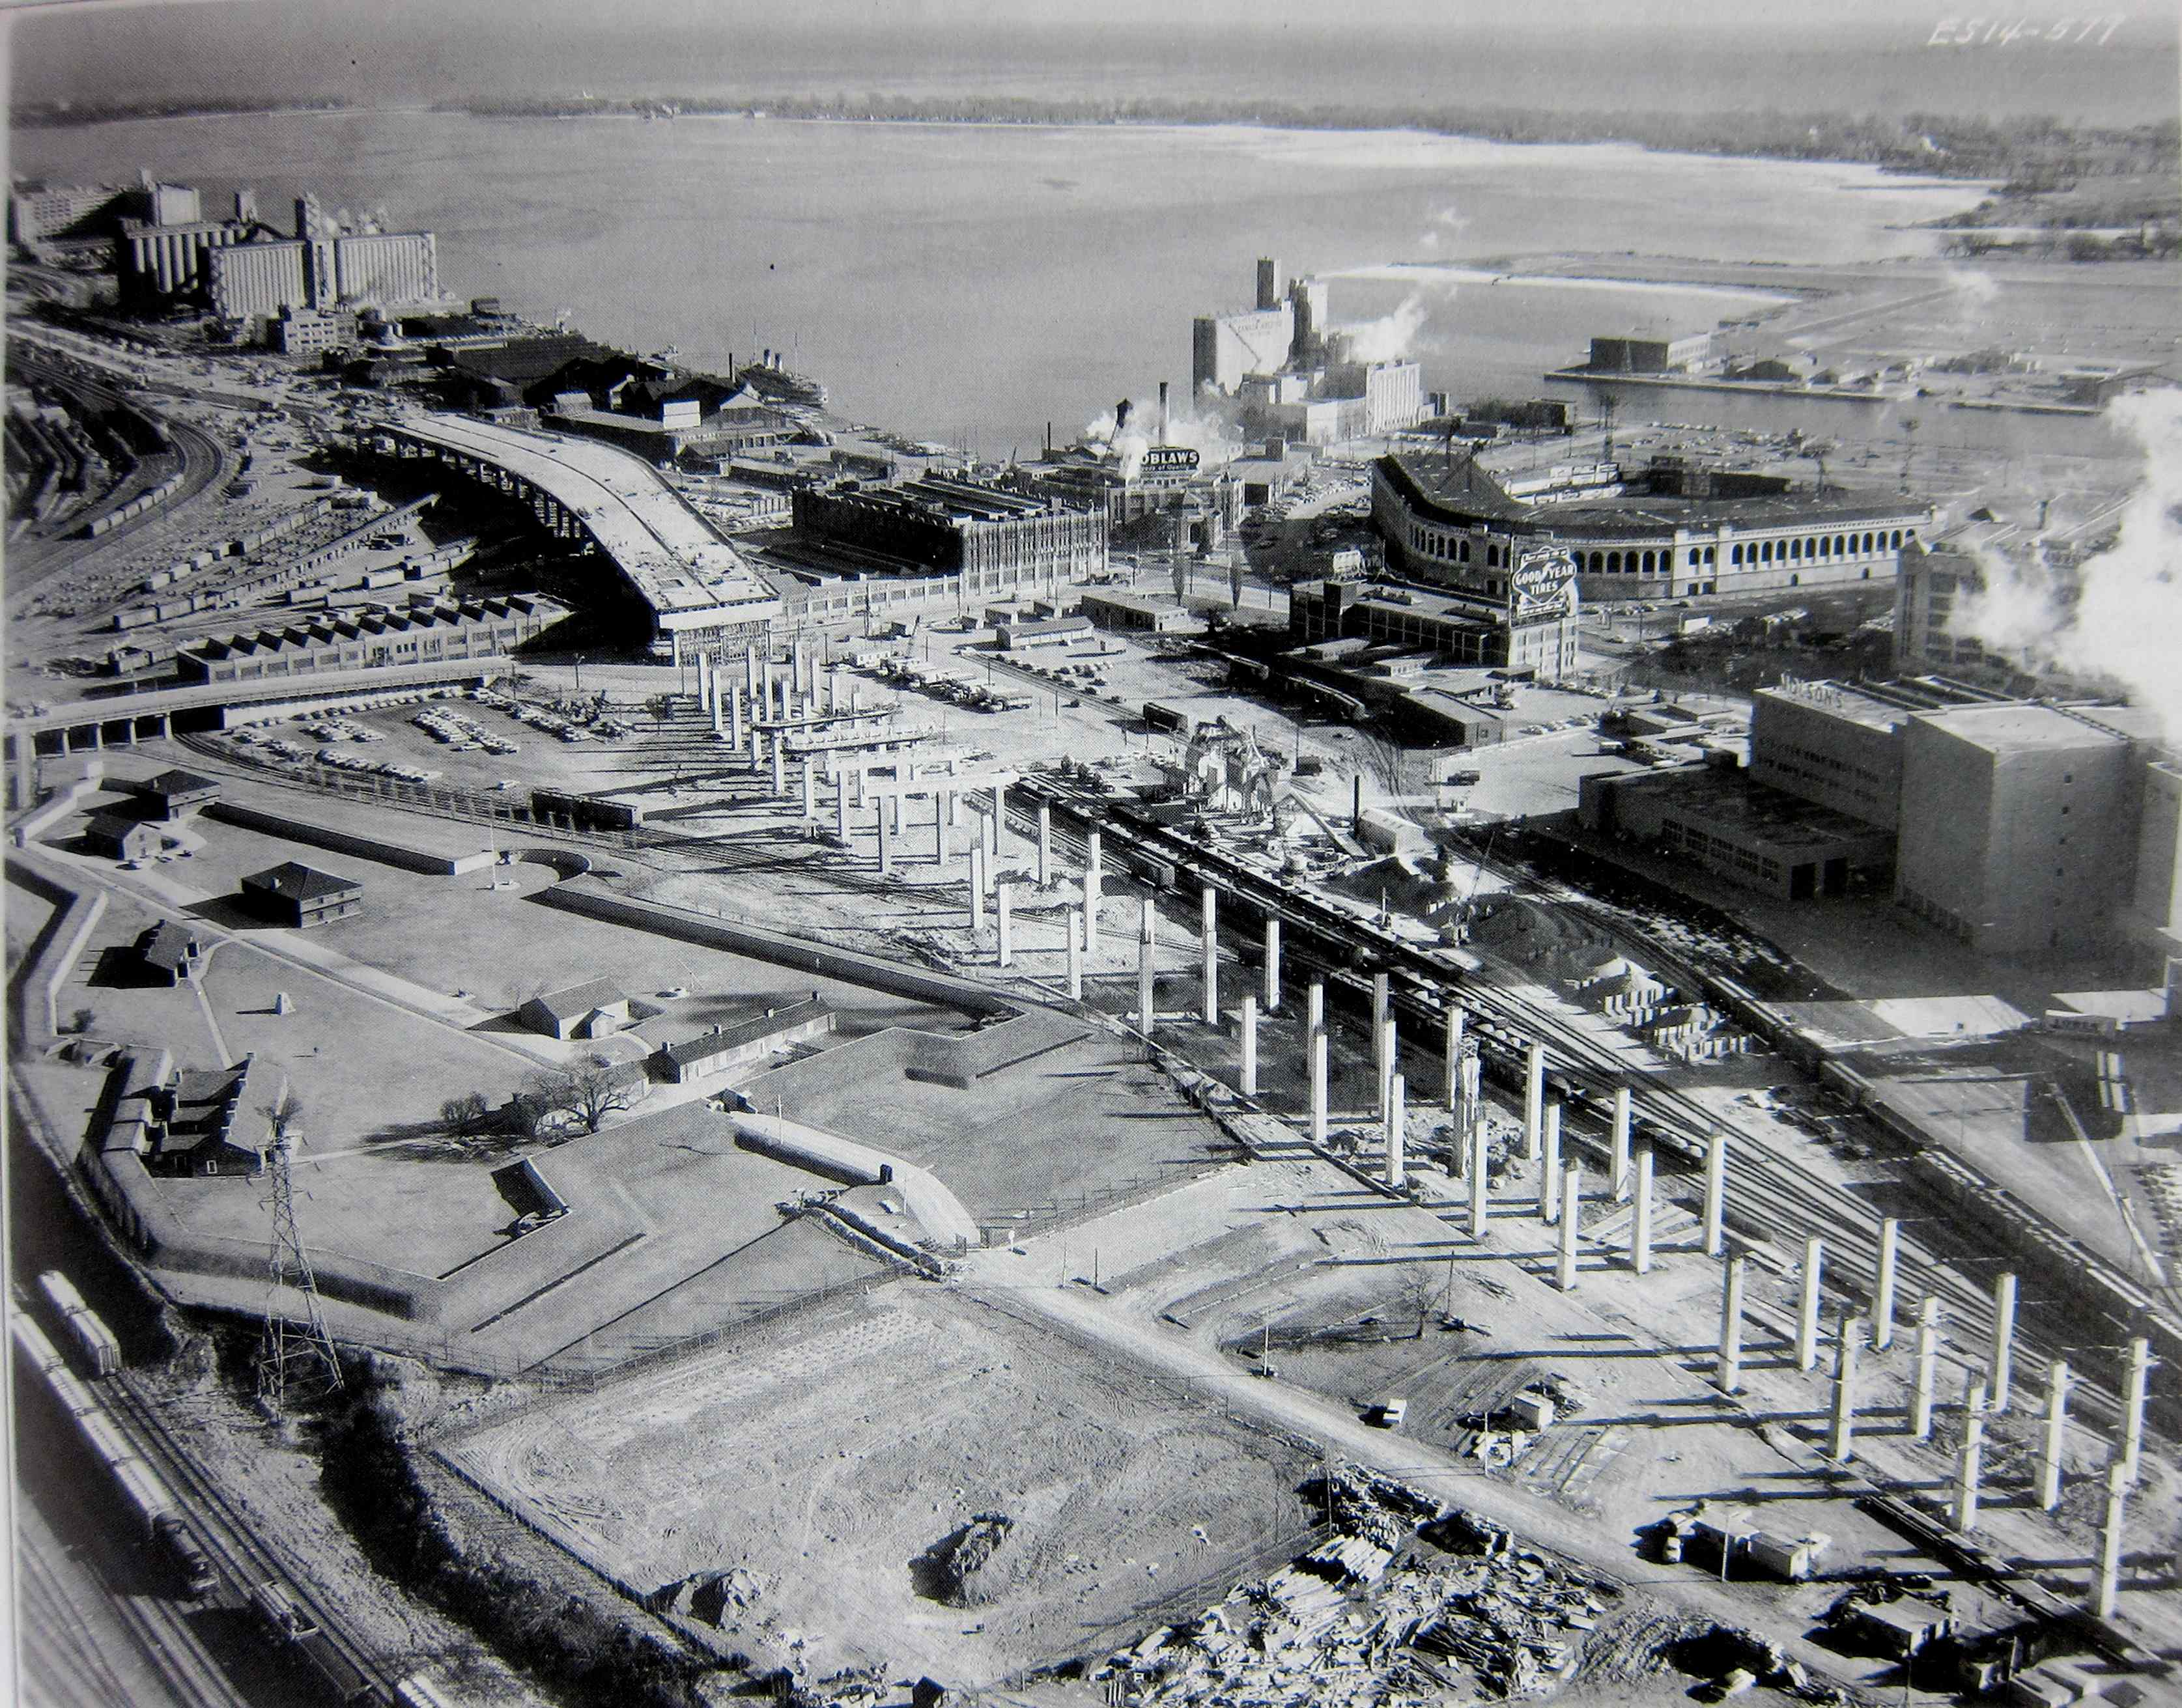
\includegraphics[width=0.7\linewidth]{images/gardiner_construction.jpg}
		
	\end{figure}
	\tiny{U of T Map and Data Library:  \url{https://maps.library.utoronto.ca/datapub/digital/NG/FY/1961GardinerExpresswayConstructionAerialFortYork.S3f189fo2xf.jpg}}
	
\end{frame}



\begin{frame}
	
	Promoting (auto)mobility - Parking!
	
	\begin{figure}
		\centering
		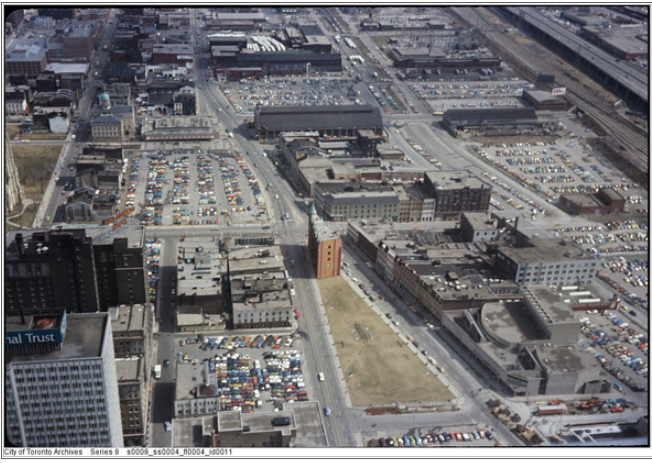
\includegraphics[width=0.7\linewidth]{images/tor_downtown_parking.png}
		
	\end{figure}
	
	
	
\end{frame}





% New arterials 1920s Vimy Circle

% Toronto highway expansion mid 20th

% Spadina subway

% Highway 413 - Bradford Bypass


\begin{frame}
	
	Promoting (auto)mobility - Corporate Interests: Retail
	
	\begin{figure}
		\centering
		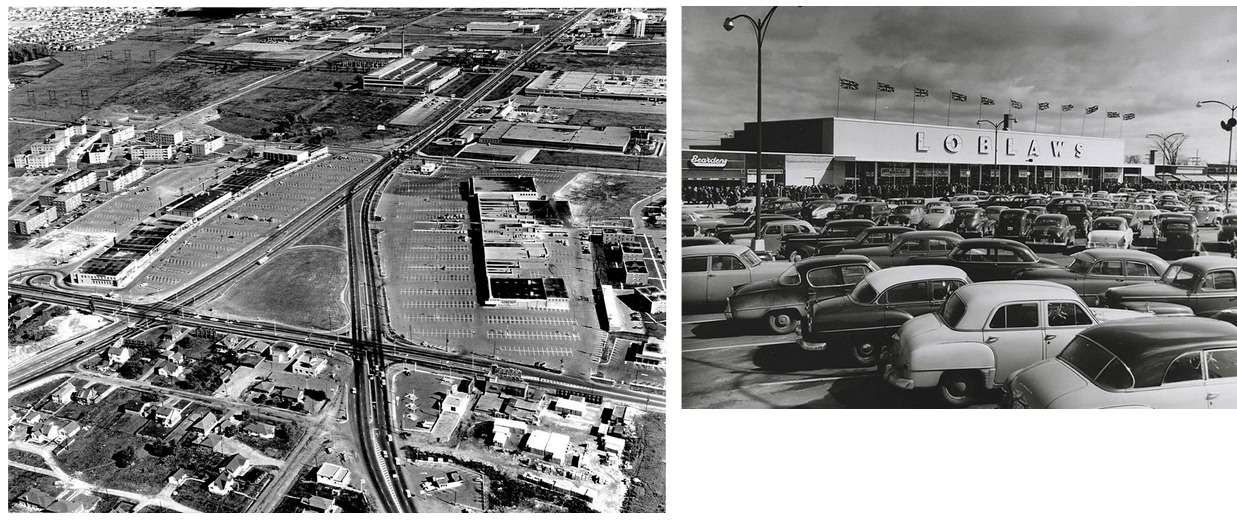
\includegraphics[width=1\linewidth]{images/golden_mile_old.png}
		
	\end{figure}

	
\end{frame}



\begin{frame}
	
	Promoting (auto)mobility - Corporate Interests: Gas Companies
	
	\begin{figure}
		\centering
		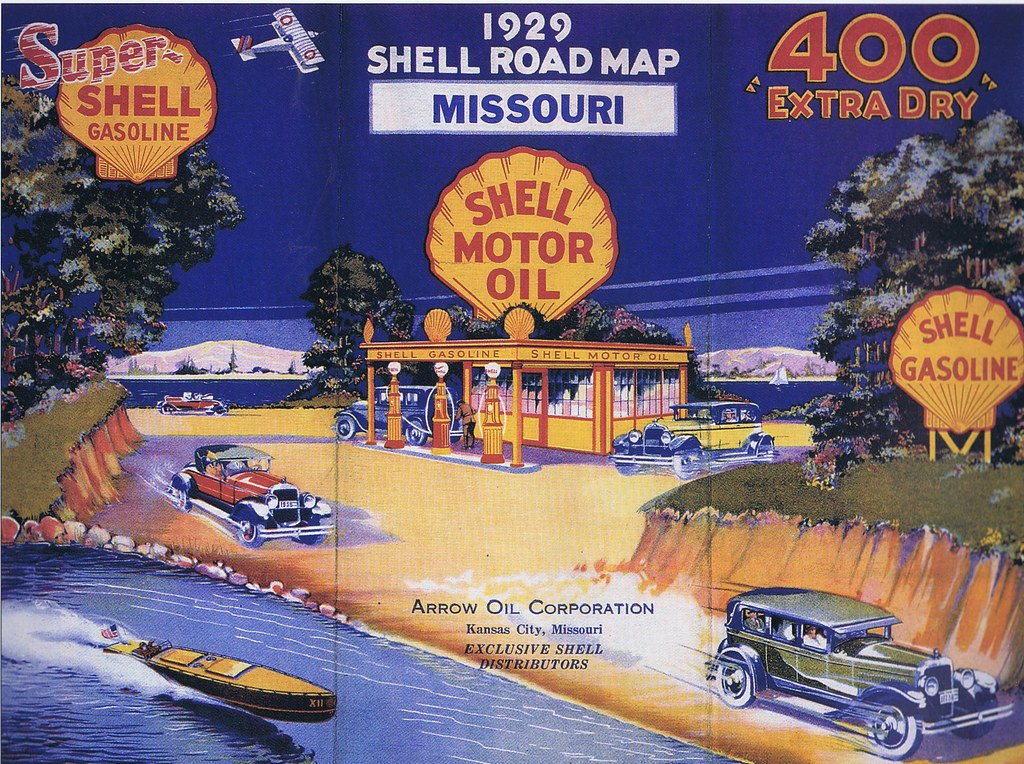
\includegraphics[width=0.75\linewidth]{images/shell_map_cover_1929.jpg}
		
	\end{figure}
	\tiny{\url{https://c1.staticflickr.com/3/2879/9378222680_a6e21d4595_b.jpg}}
	
\end{frame}




\begin{frame}
	
	\begin{figure}
		\centering
		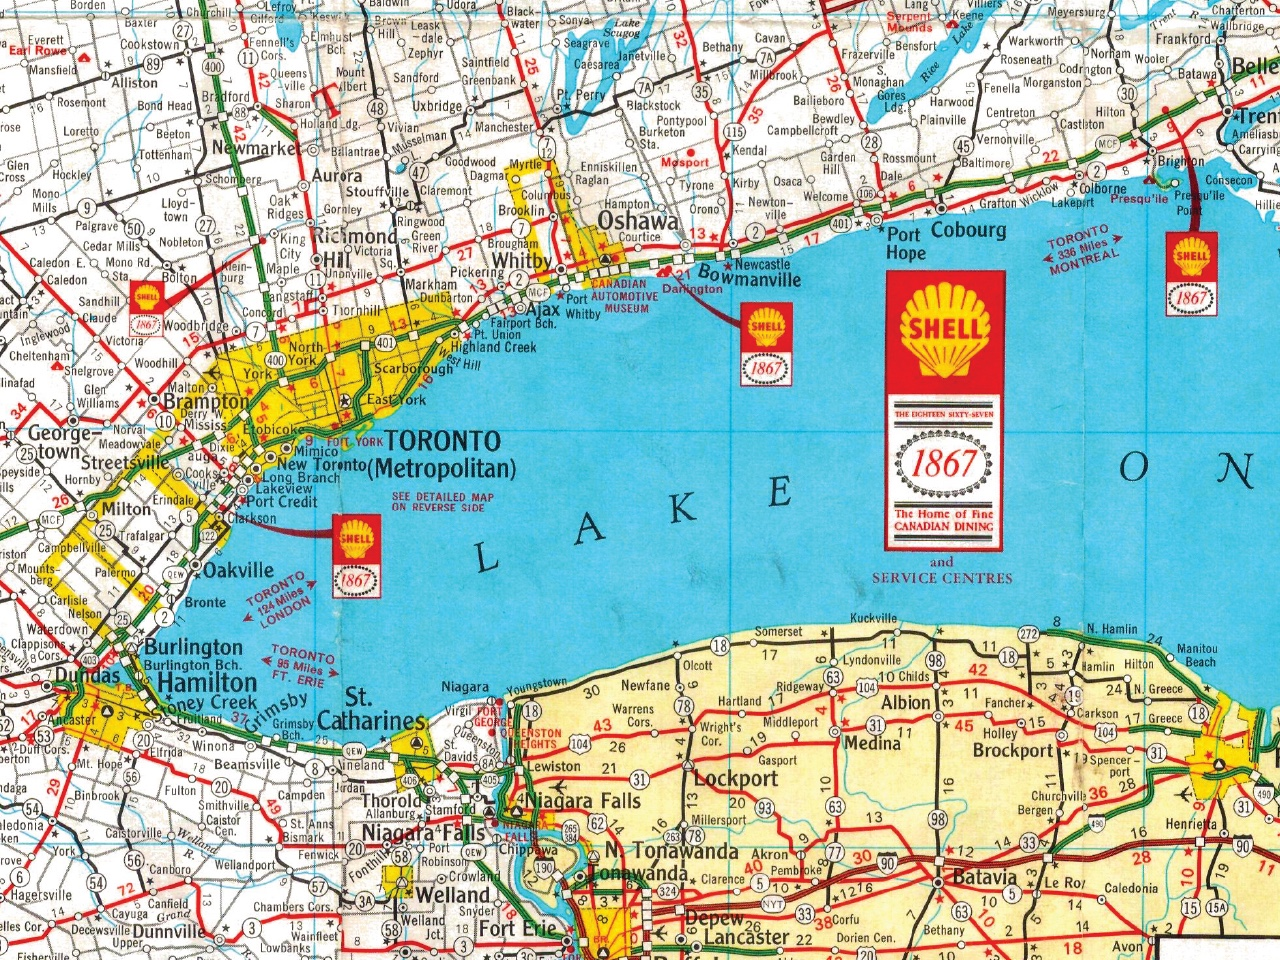
\includegraphics[width=0.85\linewidth]{images/shell_map_ontario_1968.jpg}
		
	\end{figure}
	\tiny{\url{https://www.vice.com/en/article/4xay73/the-little-known-capitalist-history-of-the-highway-map}}
	
\end{frame}


\begin{frame}
	
	 \textbf{Road Hierarchy} \\
	 
	 \begin{itemize}
	 	\item Ranking of roads based on their functions and characteristics
	 	\item Historically (and still usually) based on mobility-based attributes like vehicle speeds and throughput
	 	\item  e.g. common hierarchy
	 	\begin{enumerate}
	 		\item Highway / Motorway
	 		\item Major Arterial
	 		\item Minor Arterial
	 		\item Collector
	 		\item Local
	 	\end{enumerate}
 		\item Used for design and maintenance of road networks
	 \end{itemize}
	 

	
\end{frame}









\begin{frame}
	
	Current Road Hierarchy in Toronto:
	
	\begin{figure}
		\centering
		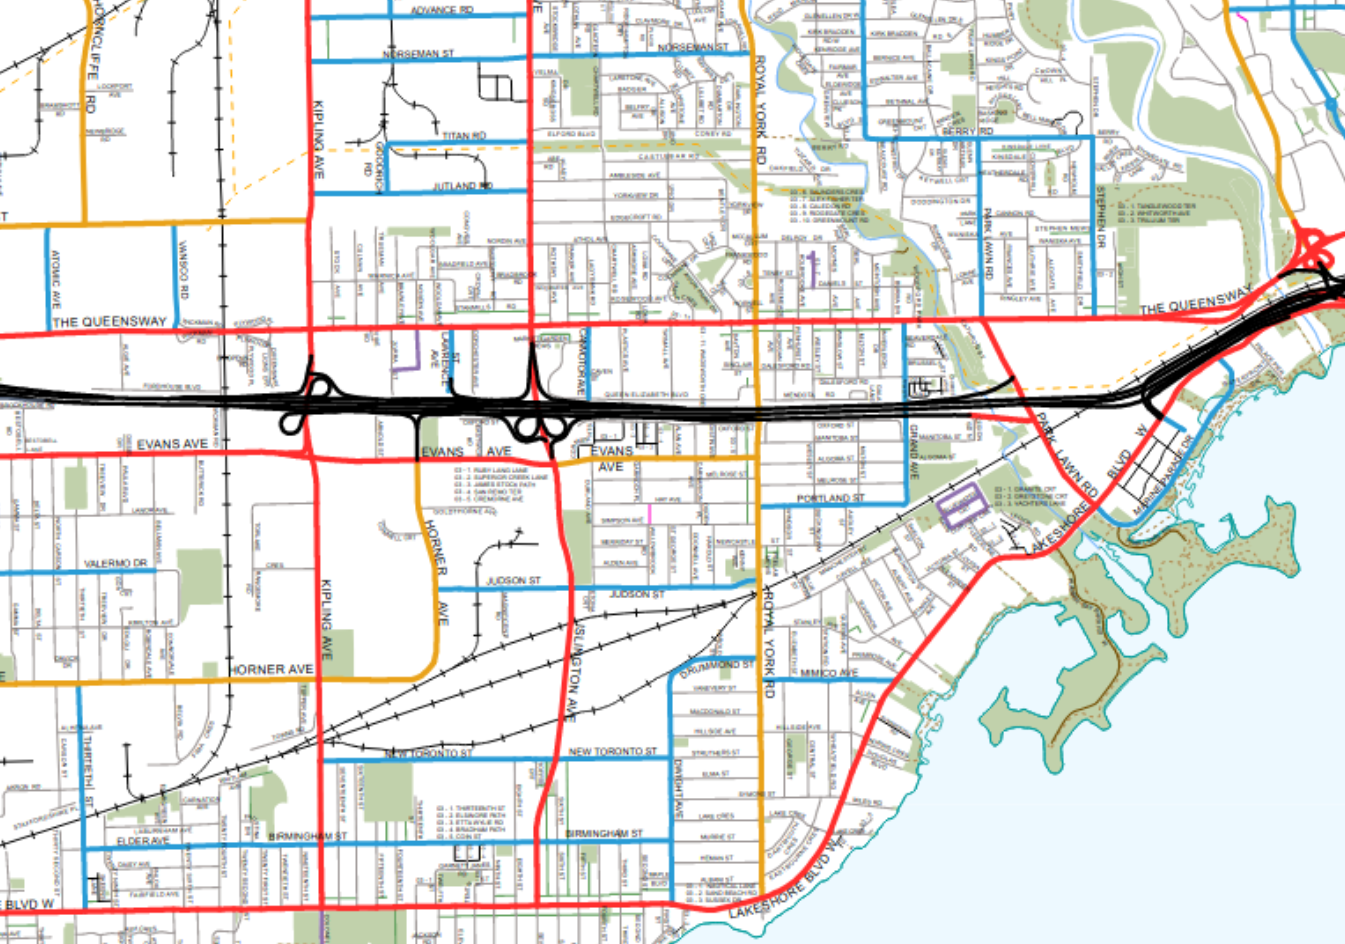
\includegraphics[width=0.85\linewidth]{images/tor_road_heir.png}
		
	\end{figure}
	\tiny{\url{https://www.toronto.ca/services-payments/streets-parking-transportation/traffic-management/road-classification-system/about-the-road-classification-system/}}
	
\end{frame}




\begin{frame}
	
	Arterial Roads = Stroads?
	
	
	\begin{figure}
		\centering
		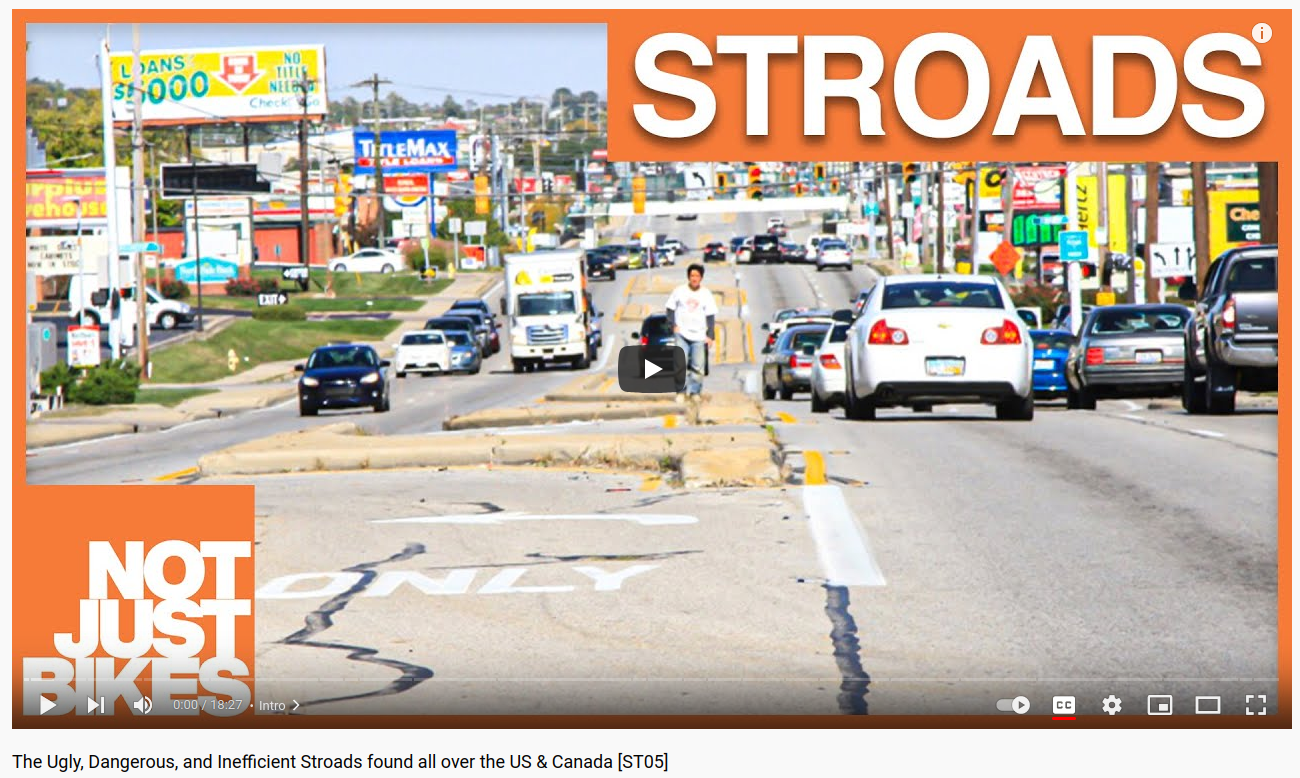
\includegraphics[width=0.85\linewidth]{images/stroads.png}
		
	\end{figure}
	\tiny{\url{https://www.youtube.com/watch?v=ORzNZUeUHAM}}
	
\end{frame}













\begin{frame}
	
	\textbf{What are the effects of expanding our road and highway networks?} 
			
	\textbf{(i.e. continuing to plan for auto-mobility)}
	
	\begin{figure}
		\centering
		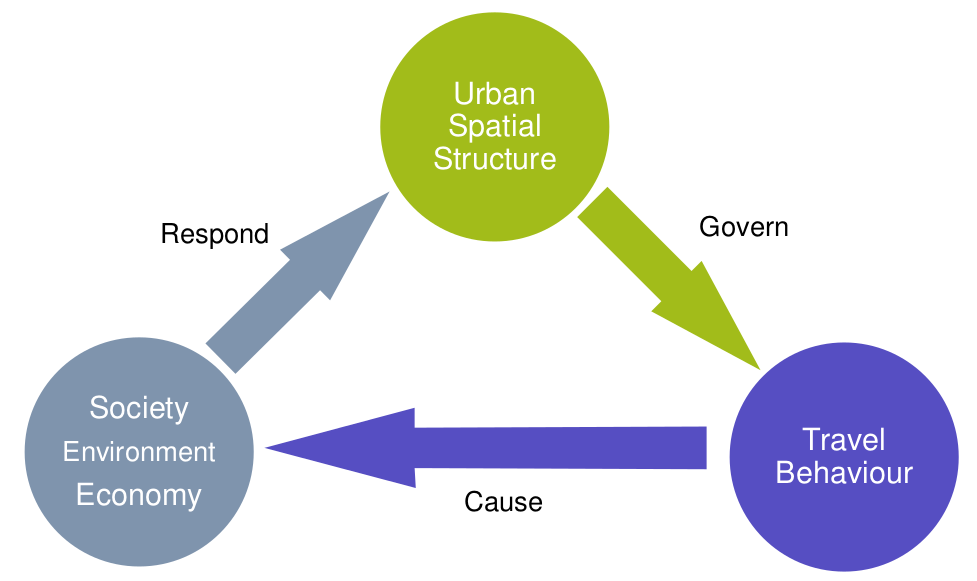
\includegraphics[width=0.79\linewidth]{images/big_links.png}
	\end{figure}
	
\end{frame}


\begin{frame}
	
	\textbf{1) What are the effects of expanding our road and highway networks on travel behaviour?}
	
	\vspace{4mm}
	
	People will drive more, but why?
	

	
\end{frame}






\begin{frame}

	\textbf{Induced demand} - as supply increases, price drops, and demand increases 
	
	\vspace{2mm}
	
	\textit{“the tailor’s remedy for obesity — letting out the seams of trousers and loosening the belt. [T]his does nothing to curb the greedy appetites that have caused the fat to accumulate.”}
	
	- Lewis Mumford
	
	\vspace{4mm}
	
	\textbf{What does this mean for transportation?}
	
	
	\vspace{8mm}
	
	
	\small See this weeks reading: \url{https://www.bloomberg.com/news/features/2021-09-28/why-widening-highways-doesn-t-bring-traffic-relief}


\end{frame}



\begin{frame}
	
	e.g. Washington Square \textbf{\textit{... attrition of automobiles}} (Jacobs, 1961)
	
	\begin{figure}
		\centering
		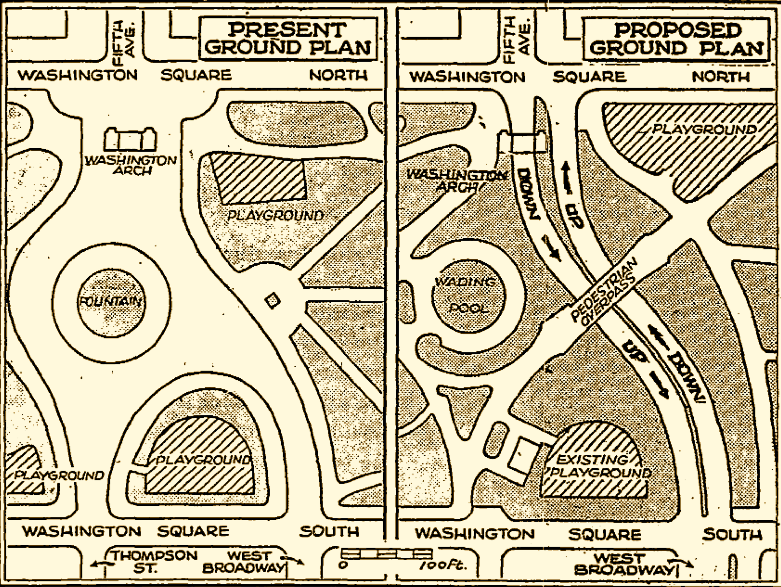
\includegraphics[width=0.65\linewidth]{images/washsquare1950splan.png}
	\end{figure}


	\tiny\url{https://ephemeralnewyork.wordpress.com/2014/04/12/the-1950s-plan-for-a-washington-square-highway/}
	
\end{frame}






\begin{frame}
	\begin{columns}
		\begin{column}{0.5\textwidth}
			
			\textbf{\textit{Erosion of cities ...} }
			
			(Jacobs, 1961)
			
			\vspace{8mm}
			
			
			
			\small
			Also see Robinson, R. (2011) The Spadina Expressway Controversy in Toronto, Ontario. \textit{Canadian Historical Review}
			
			
			\vspace{8mm}
			
			\tiny Image source: \textit{The BAD TRIP, The Untold Story of the Spadina Expressway}
			
			
			
		\end{column}
		
		\begin{column}{0.5\textwidth}
			\begin{figure}
				\centering
				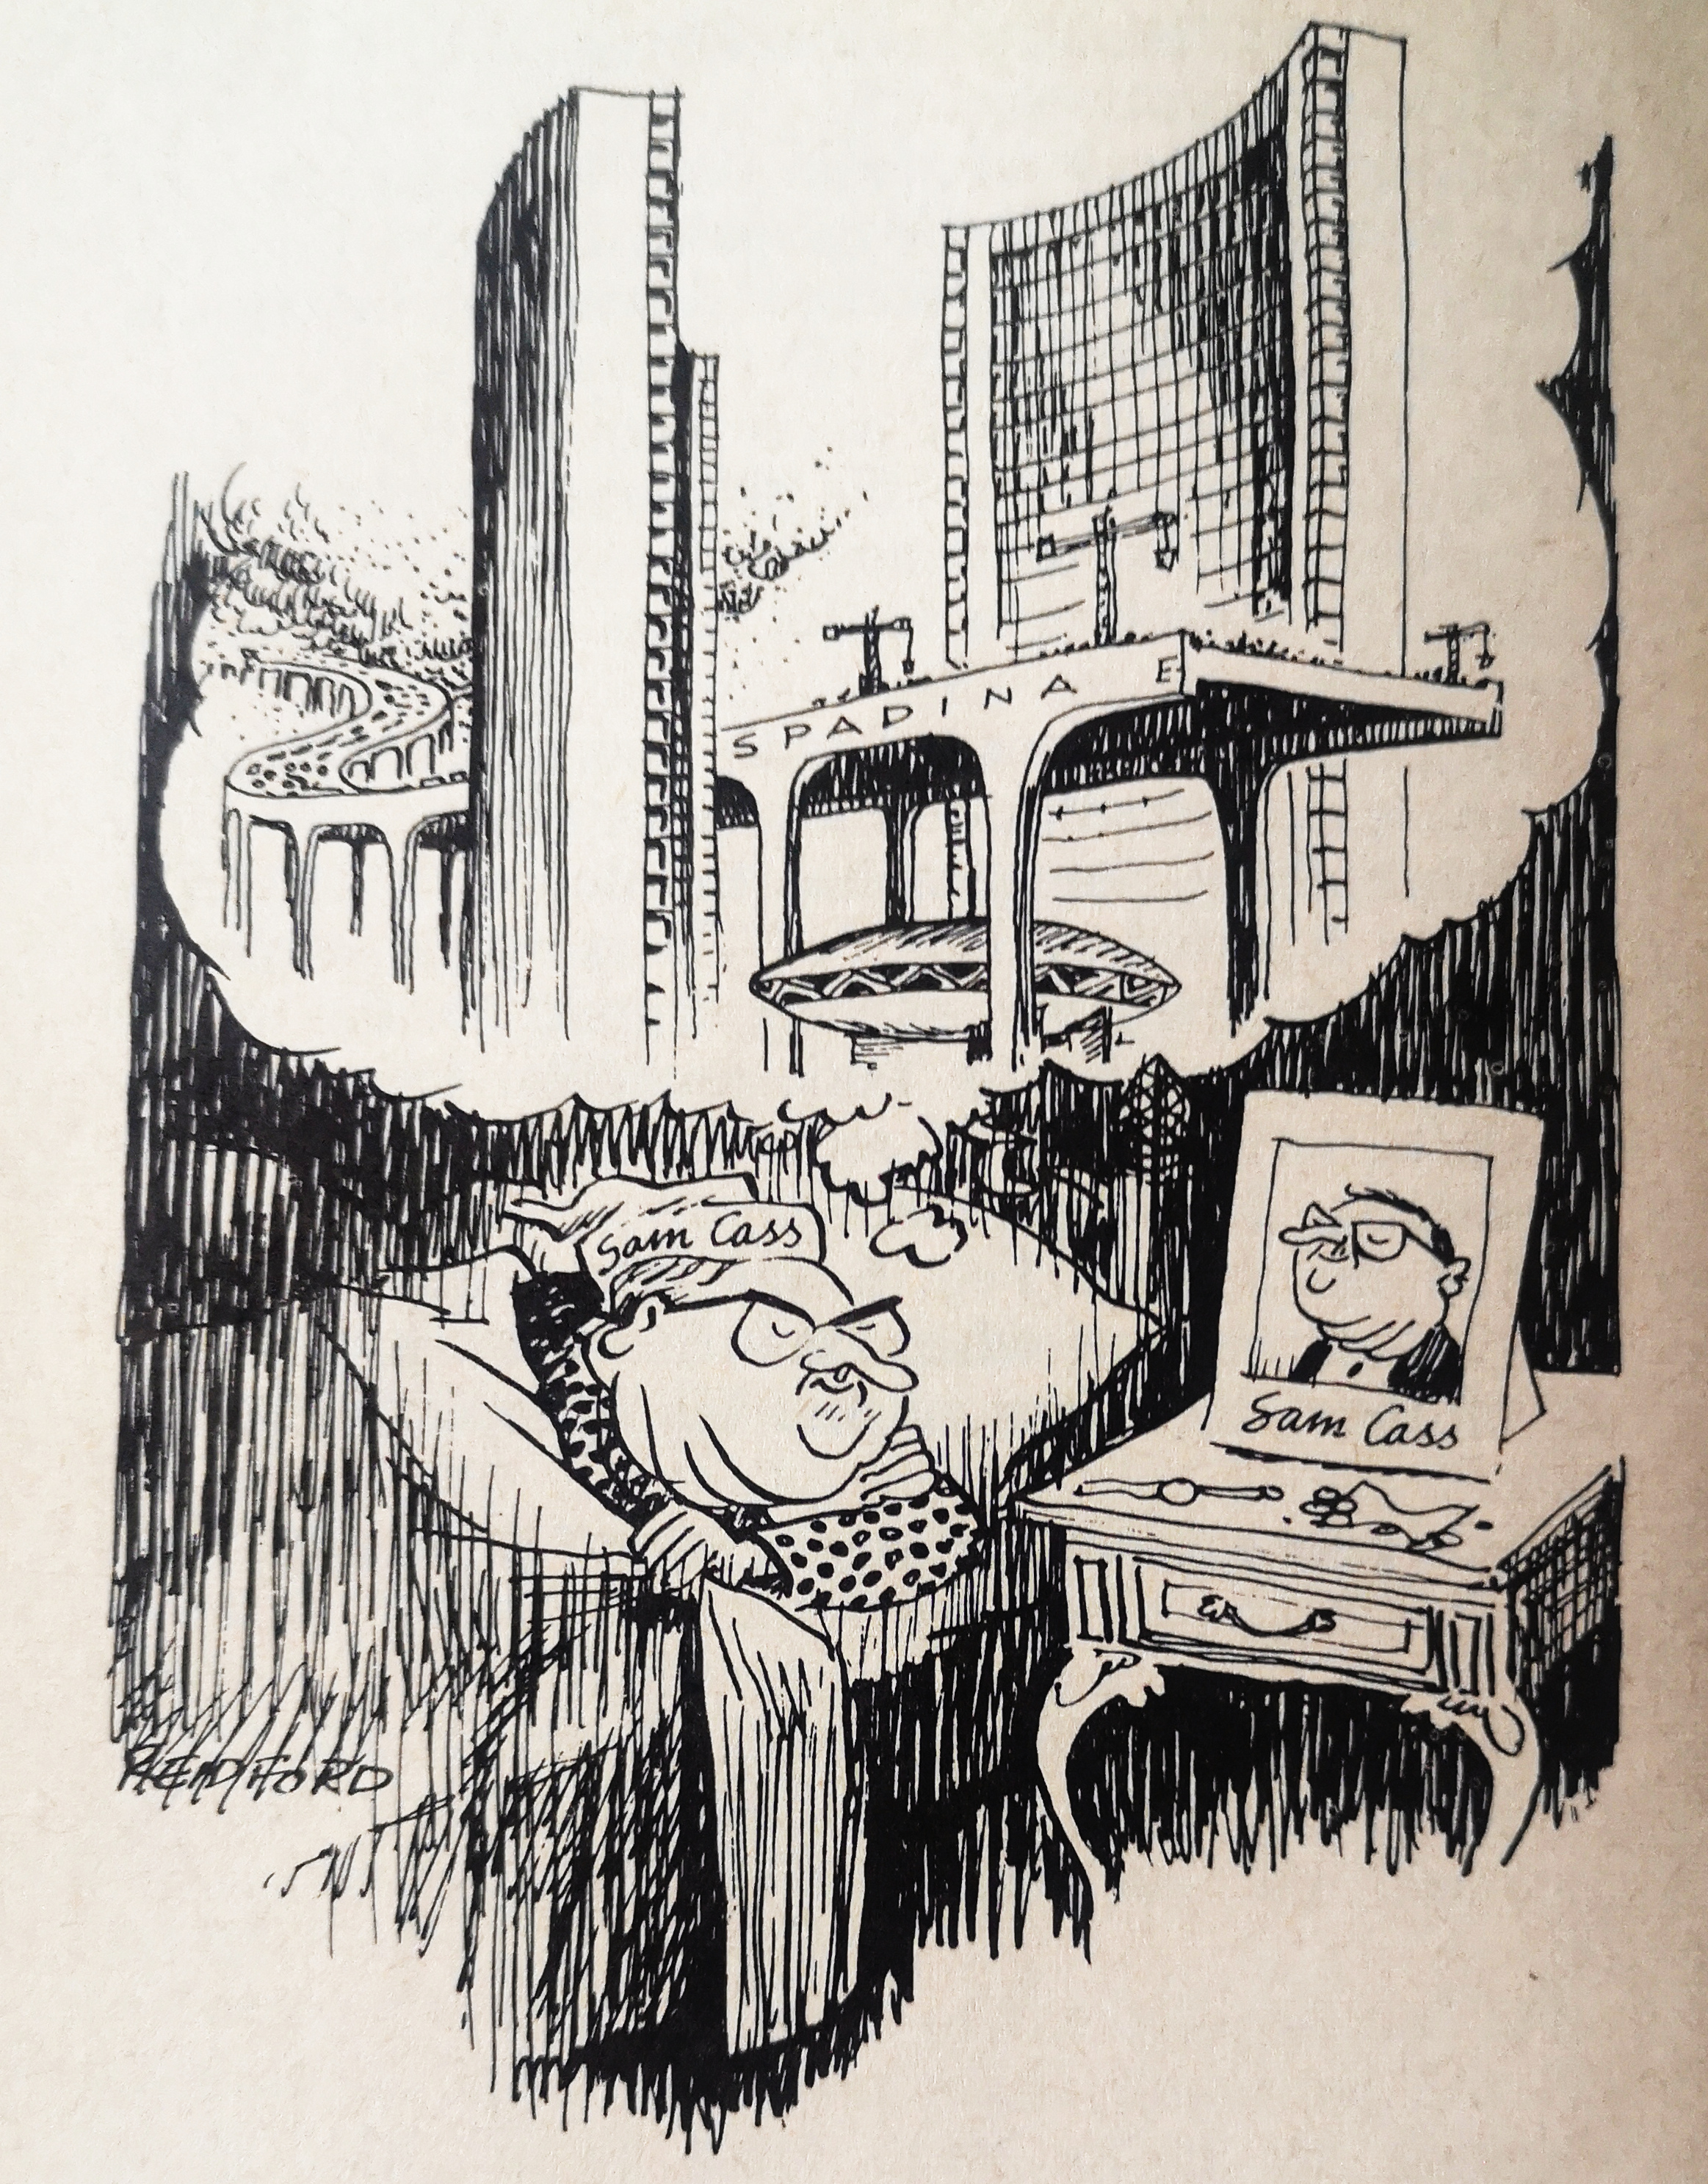
\includegraphics[width=1\linewidth]{images/spadina_cartoon.jpg}
			\end{figure}
			
		\end{column}
		
		
		
	\end{columns}
\end{frame}








\begin{frame}
	
	Positive Feedback Loops:
	
	\begin{figure}
		\centering
		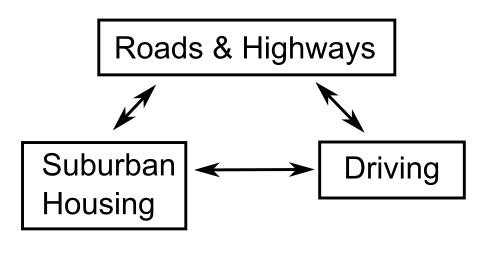
\includegraphics[width=0.4\linewidth]{images/feedback_suburb_driving.png}
	\end{figure}

	Research example: \small\url{https://www.jstor.org/stable/25098858}

\begin{figure}
	\centering
	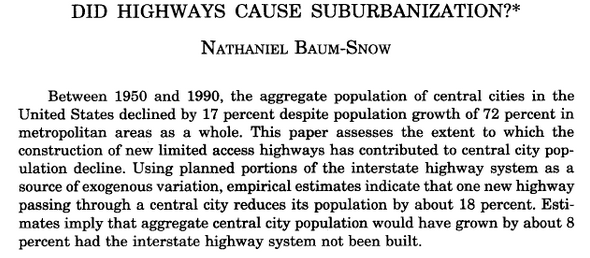
\includegraphics[width=0.7\linewidth]{images/baumsnow_highways.png}
\end{figure}
		
\end{frame}

	
	
\begin{frame}
	
	\begin{figure}
		\centering
		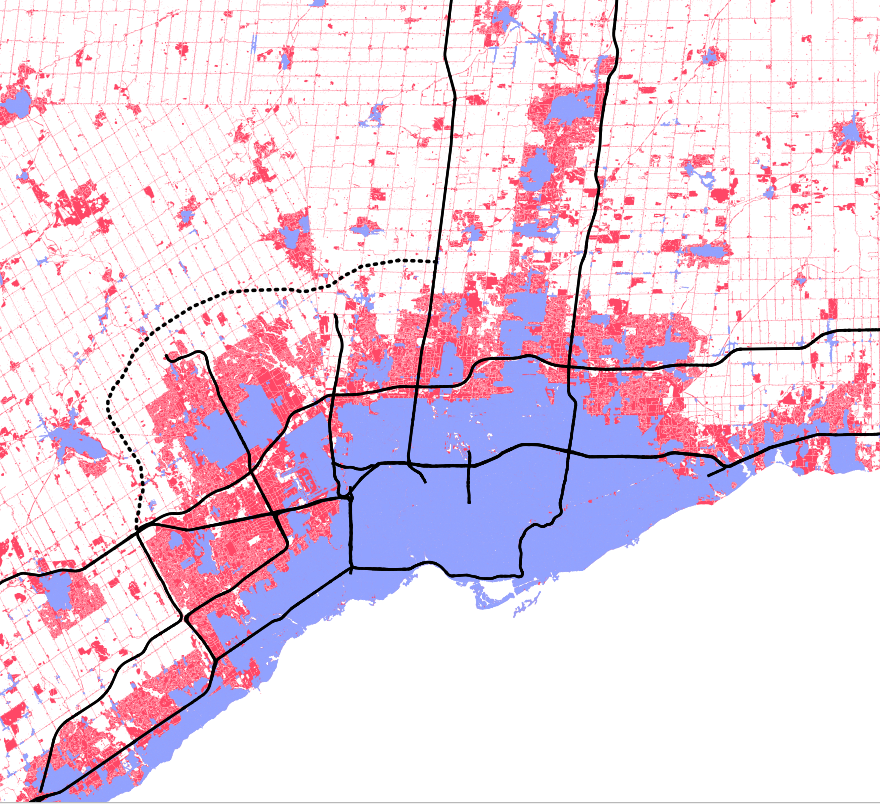
\includegraphics[width=0.7\linewidth]{images/highways_dev_toronto.png}
	\end{figure}
	
\end{frame}
	



\begin{frame}
	
	Debates over new highways continue ...
	
	\begin{figure}
		\centering
		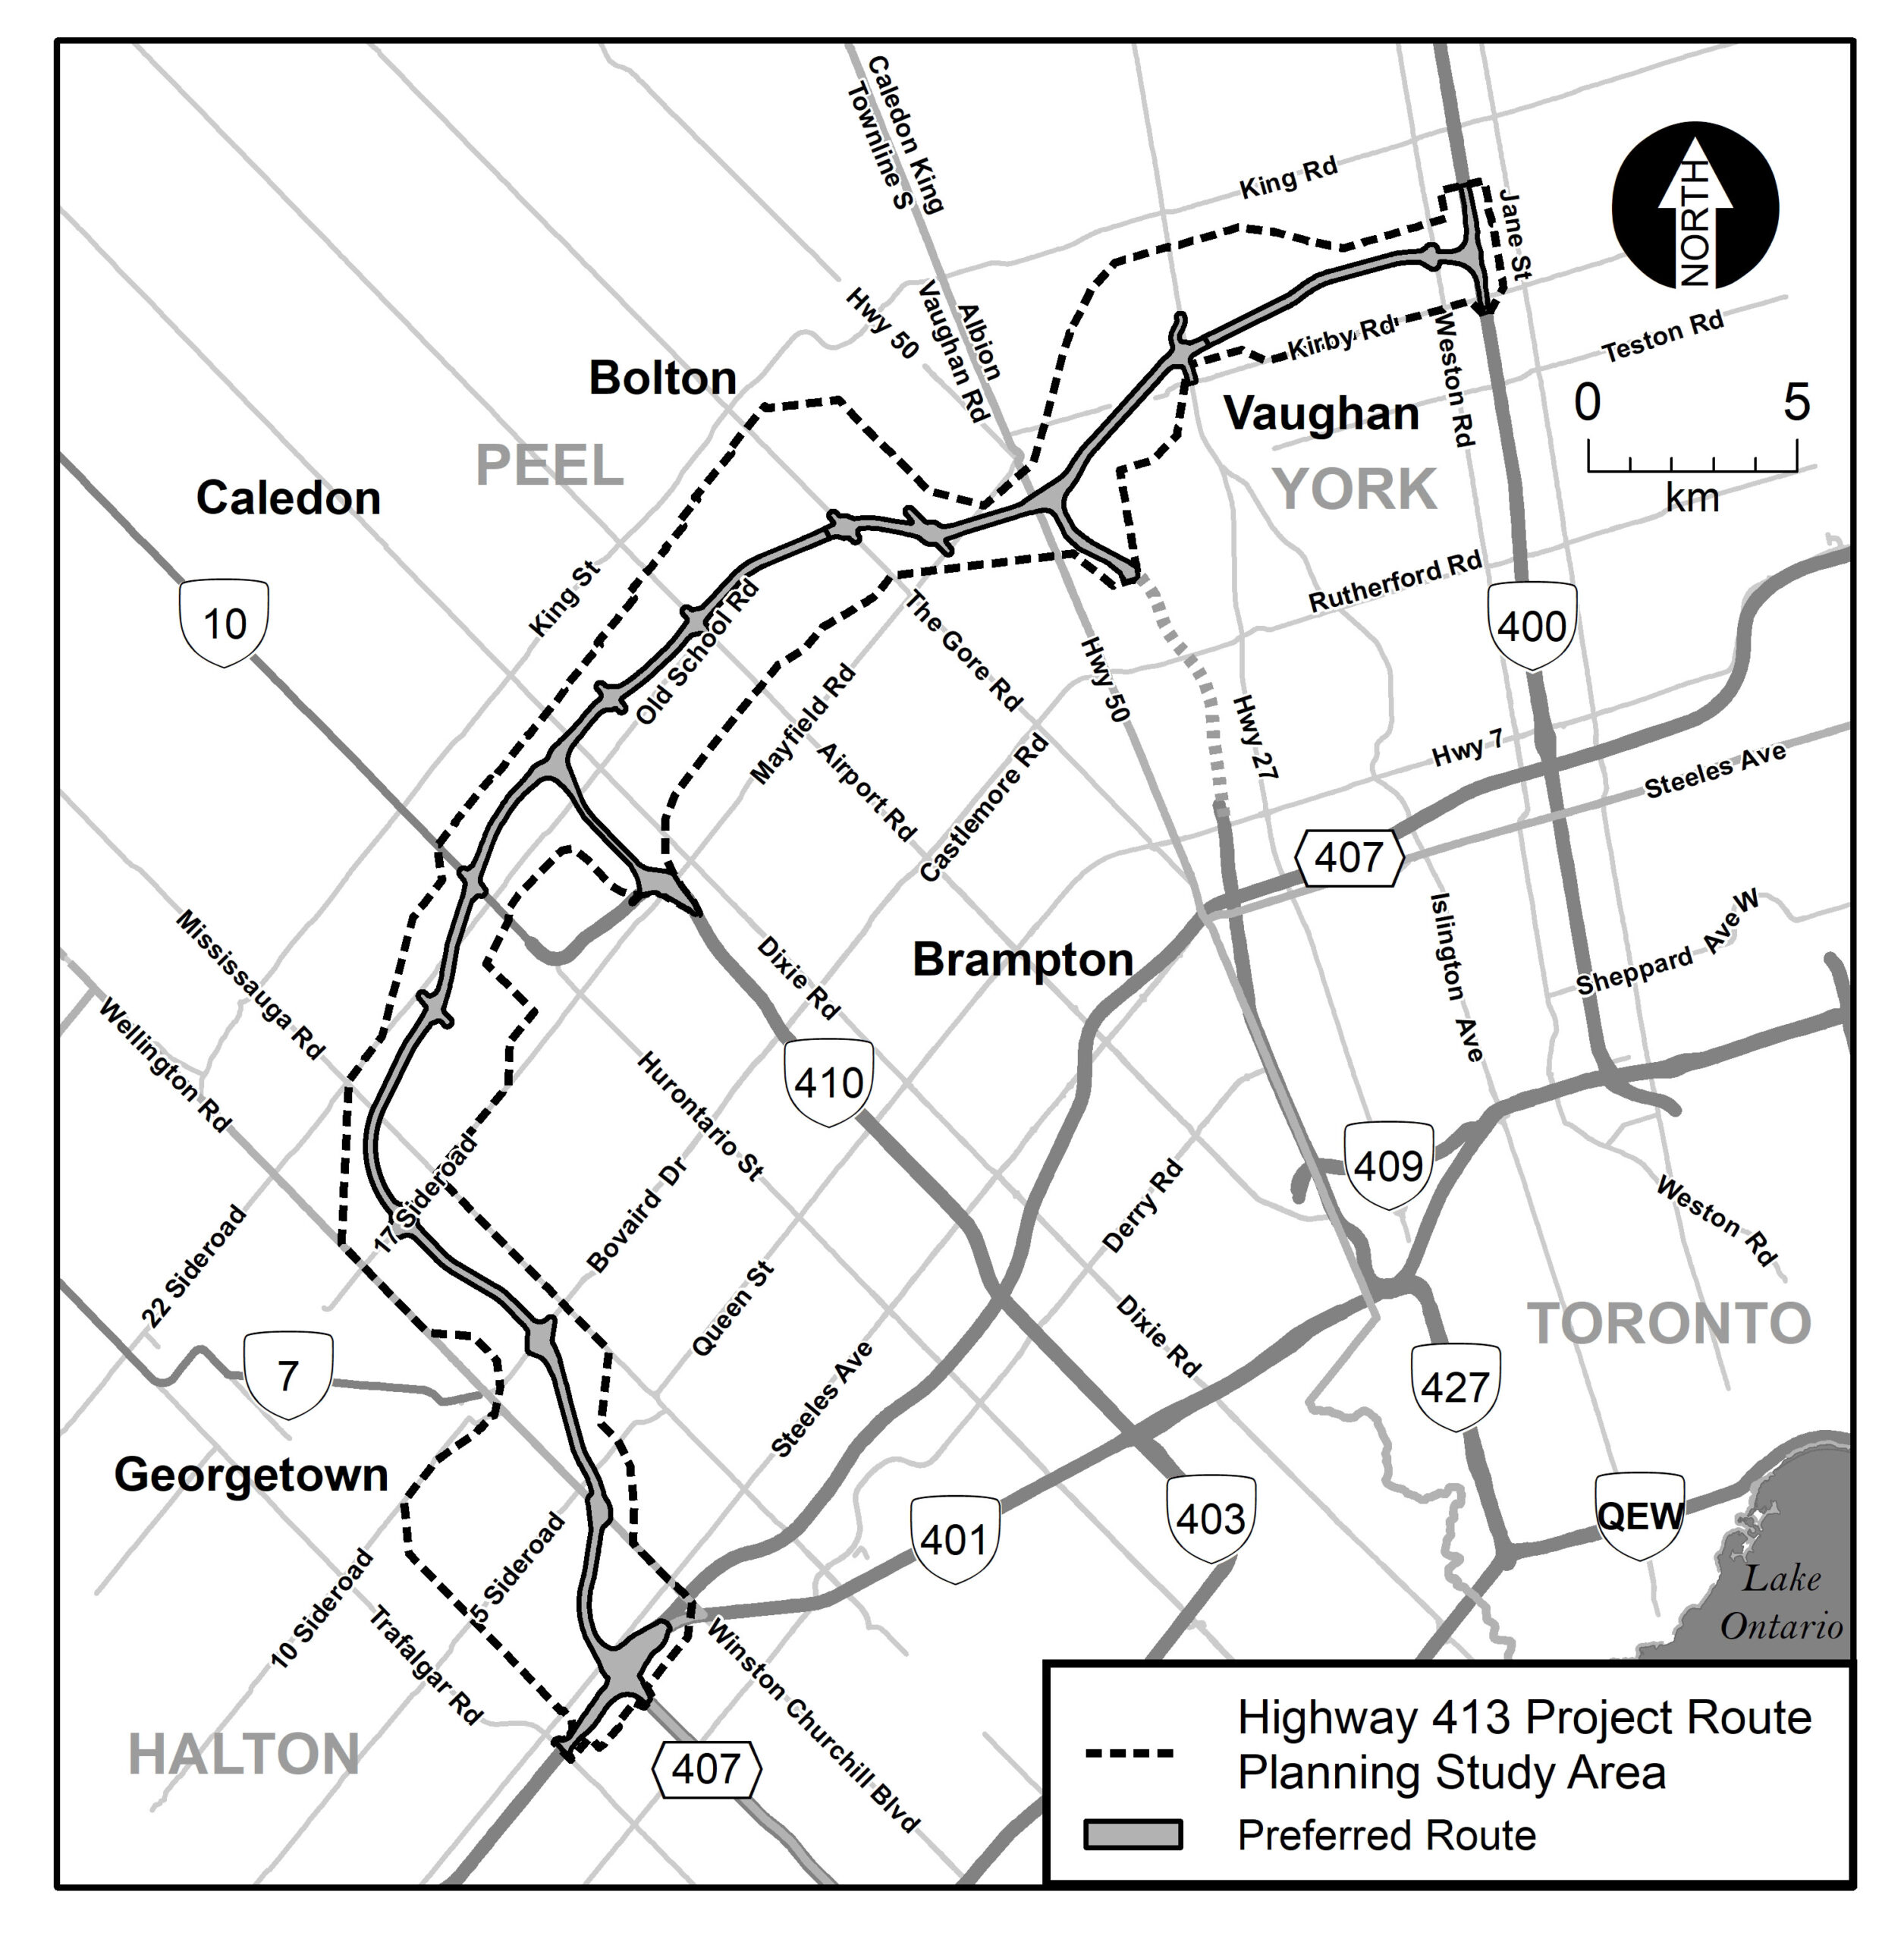
\includegraphics[width=0.45\linewidth]{images/highway413.jpg}
		
	\end{figure}
	\tiny{\url{https://www.highway413.ca/}}
	
	\vspace{1mm}
	
	 \url{https://www.inthehills.ca/wp-content/uploads/2020/11/413_GTA_WestCorridor14_withLEGEND_CORRECTED.jpg}
	\vspace{1mm}
	
	\tiny{TVO (2018) Highways and our Transportation Future \url{https://www.tvo.org/video/highways-and-our-transportation-future}} 
	
\end{frame}
	
	




\begin{frame}
	
	\textbf{Administration of roads and highways}
	
	\vspace{2mm}
	
	Usually tiered by government, e.g. in Ontario:
	
	\begin{enumerate}
		
		\item Government of Ontario, Ministry of Transportation (MTO)
		\begin{itemize}
			\item 400 Series Highways
			\item "King's" Highways - "primary" highways (i.e. major rural routes)
			\item 500/600 "secondary" highways (mainly in Northern Ontario)	
		\end{itemize}
	
		\item Local Governments (\textit{Transportation Services} in Toronto)
		\begin{itemize}
			\item Most Local Roads (e.g. see road hierarchy in previous slide)
			\item Can include private access highways (e.g. DVP)
		\end{itemize}
		
	\end{enumerate}
	
\end{frame}



\begin{frame}
	
	Ontario highways in red:
	
		\begin{figure}
			\centering
			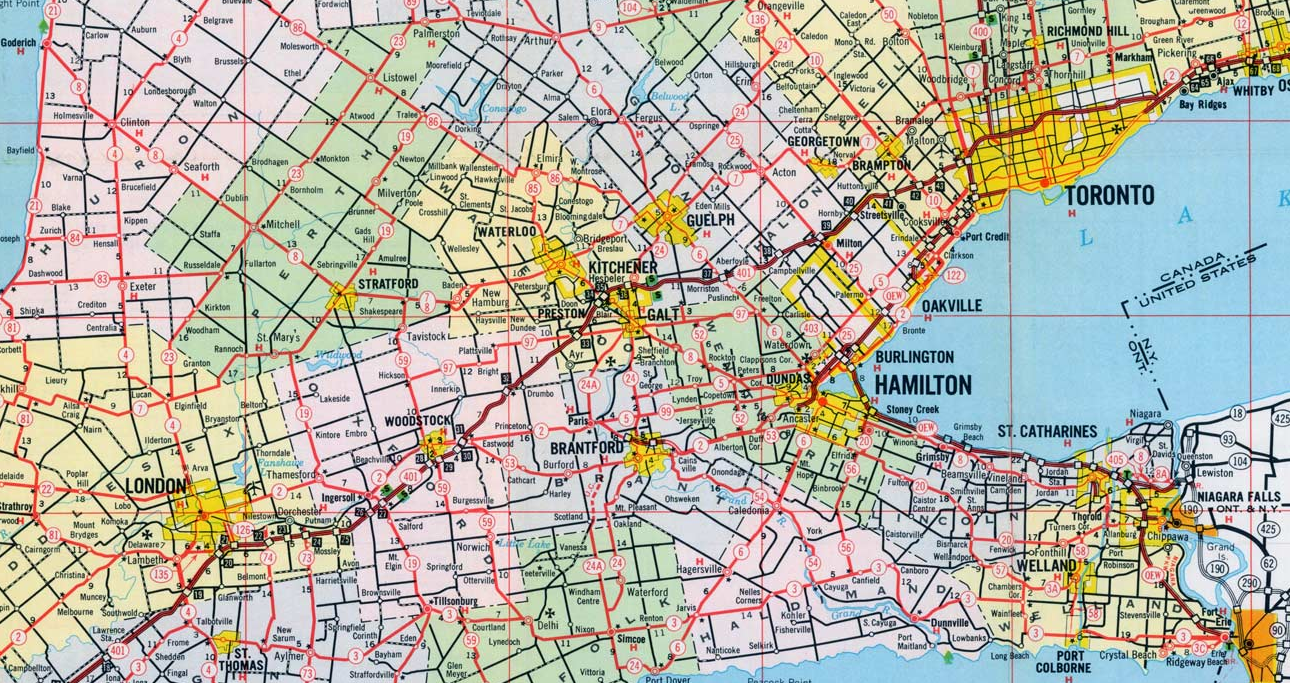
\includegraphics[width=1\linewidth]{images/ontario_road_map.png}
		\end{figure}
	
	\tiny\url{http://www.thekingshighway.ca/}

\end{frame}





\begin{frame}
	
	Common responsibilities of local and provincial transportation authorities
	
	\begin{itemize}
		\item Daily maintenance
		\item Resurfacing
		\item Signage and traffic signals
		\item Street furniture / sidewalks
		\item On-street parking
		\item On-street patios
		\item Redesign / reconstruction
		\item Planning \& designing new infrastructure
		\item And more!
	\end{itemize}
	
\end{frame}


\begin{frame}
	
	e.g. snow plowing in Toronto
	
	\begin{figure}
		\centering
		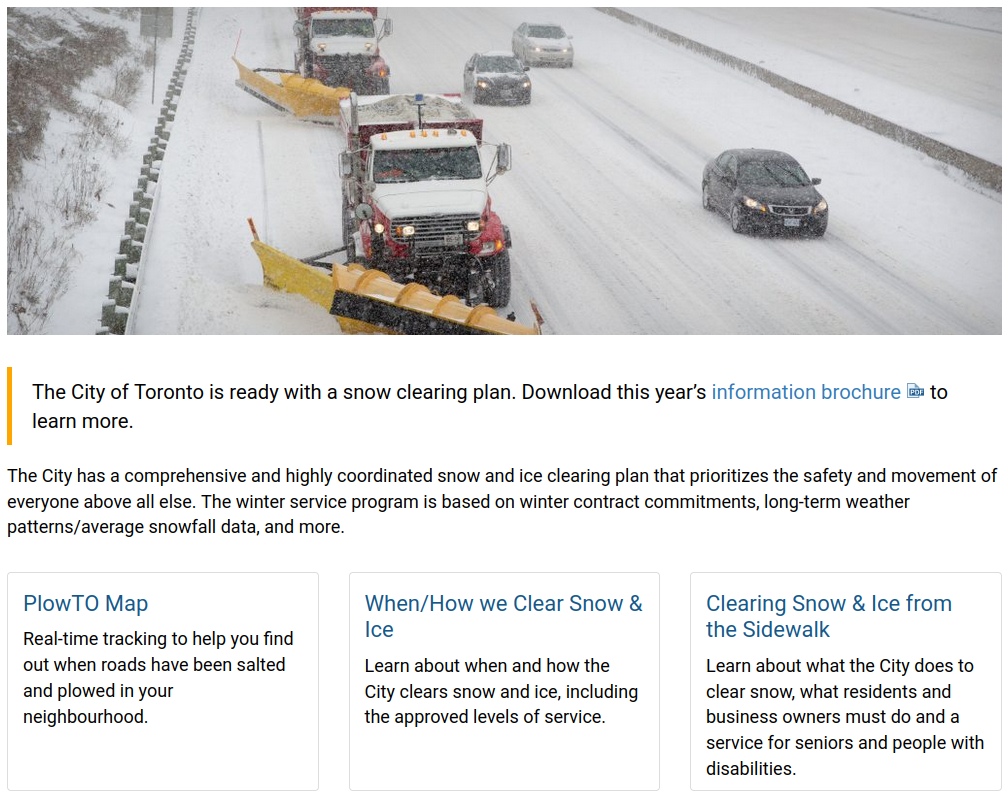
\includegraphics[width=0.7\linewidth]{images/winter_to.png}
	\end{figure}

	\tiny\url{https://www.toronto.ca/services-payments/streets-parking-transportation/road-maintenance/winter-maintenance/}
	
\end{frame}





\begin{frame}
	e.g. road redesign and construction
	
	\begin{figure}
		\centering
		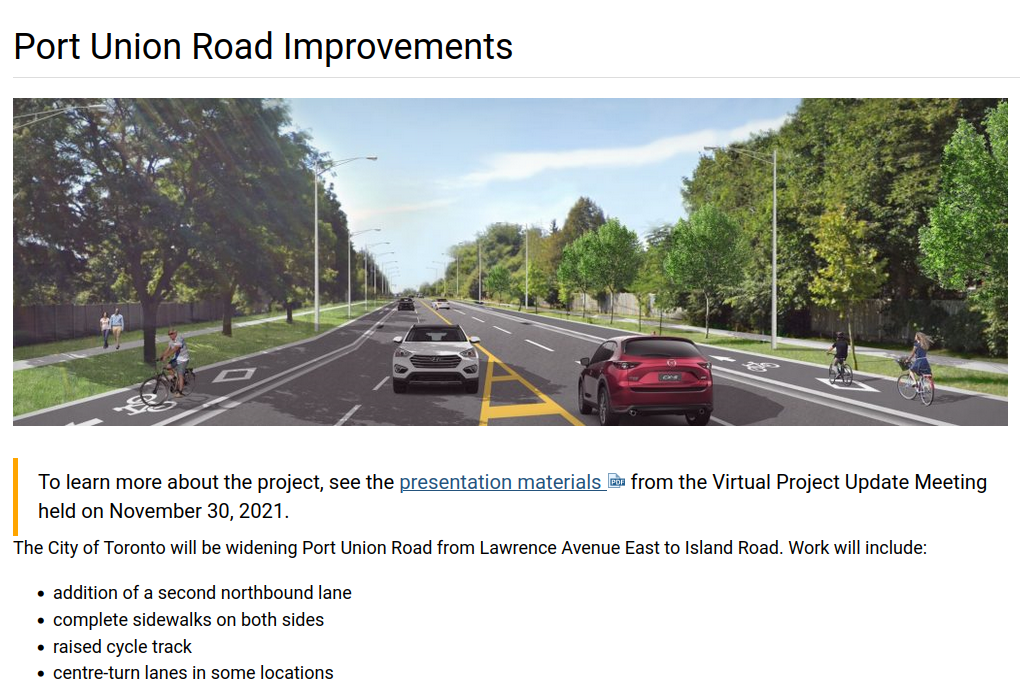
\includegraphics[width=0.7\linewidth]{images/port_union.png}
	\end{figure}
	
	\tiny\url{https://www.toronto.ca/community-people/get-involved/public-consultations/infrastructure-projects/portunionroad/}
\end{frame}






\begin{frame}
	
	
	
	\begin{columns}
		\begin{column}{0.7\textwidth}
			
			Case Study: \textbf{Don Valley Parkway}
	
			\begin{itemize}
				\item Major auto route into downtown Toronto
				\item 3 lanes in each direction, 12 exits
				\item Approximately 135,000 (weekday average) vehicles per day
				\item Original design of only 60,000 vehicles per day
				\item Ample congestion (i.e. high social and economic costs)
				\item Traverses environmentally sensitive area (Don Valley)
			\end{itemize}

		\end{column}

	\begin{column}{0.3\textwidth}
		
		\begin{figure}
			\centering
			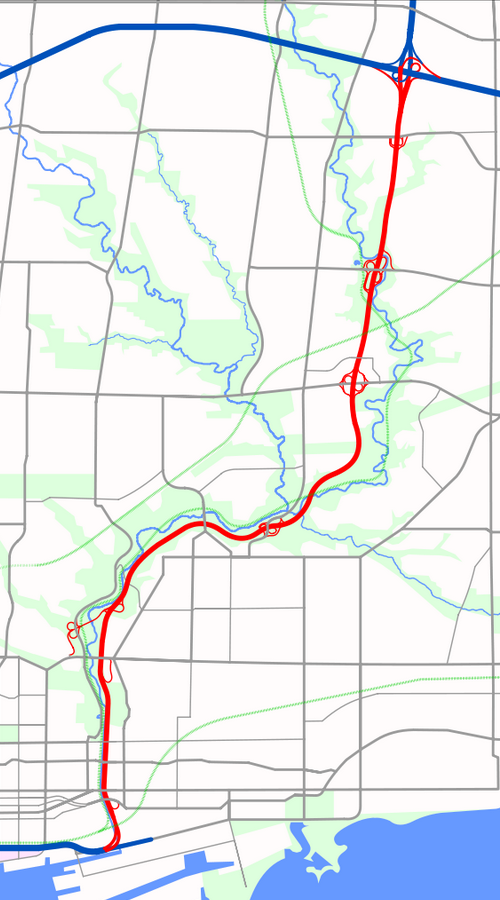
\includegraphics[width=1\linewidth]{images/dvp_map_wiki.png}
		\end{figure}
		
		
	\end{column}



\end{columns}
		
\end{frame}



\begin{frame}
	\begin{columns}
		\begin{column}{0.5\textwidth}
			
			\textbf{Options for the Don Valley Parkway:}
			
			\begin{enumerate}
				\item Maintain
				\item Adapt, by adding tolls/congestion charges
				\item Adapt, by increasing transit capacity
				\item Widen highway
				\item Remove entirely
				\item Other/Combination
			\end{enumerate}
			
		\end{column}
		
		\begin{column}{0.5\textwidth}
			\begin{figure}
				\centering
				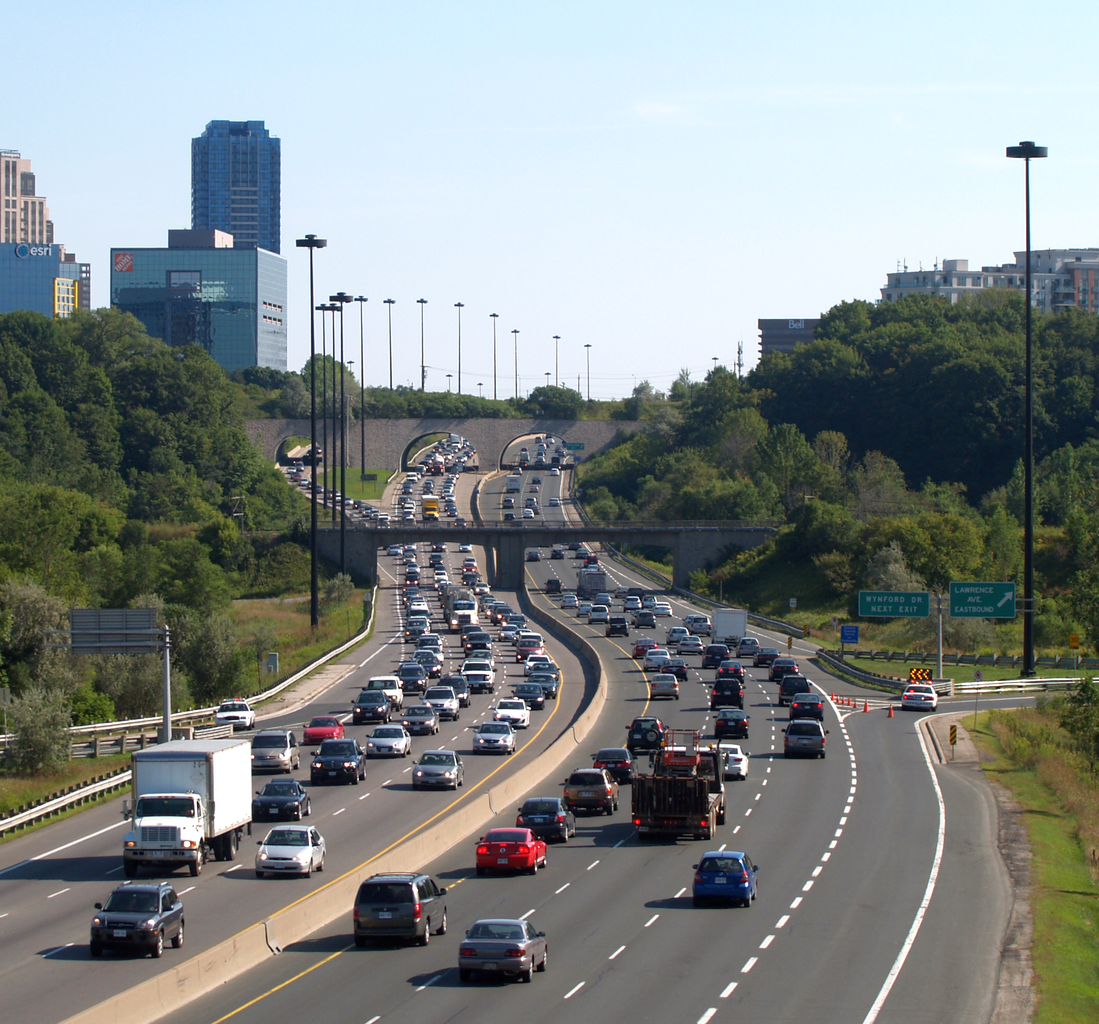
\includegraphics[width=1\linewidth]{images/dvp_congestion_2014.png}
			\end{figure}
			
		\end{column}
		
		
		
	\end{columns}
\end{frame}






\begin{frame}
	\textbf{Next Week} 
	
	\vspace{4mm}
	
	Cycling \& Walking:
	
	\begin{itemize}
		
		
		
		\item Walking and cycling in the city
		
		\item Health benefits of active travel
		
		\item Safety issues
		
		\item Streets as public spaces
		
		\item Designing "complete streets"
		
		
		
	\end{itemize}

\end{frame}




\end{document}